% ********************************** %
% UNIVERSITE PARIS 8
% INSTITUT D'ENSEIGNEMENT À DISTANCE
% L1 LICENCE INFORMATIQUE 
% 2023 - 2024
     
% OUTILS COLLABORATIFS (TP(S)) %

% NOM: PULUDISU Mpia Mimpiya
% Numéro étudiant: 18913467
% ********************************** %

% Initialisation du document de type "article"
% format A4 et des marges de 1.8 cm sur chaque côté.
\documentclass[a4paper,11pt]{article}
\usepackage[a4paper, margin=1.8cm]{geometry}
% Encodage de caractère
\usepackage[T1]{fontenc} 
% Définit l'encodage UTF-8
\usepackage[utf8]{inputenc}
% Permet la gestion des particularités linguistiques 
% propres à la langue française
\usepackage[french]{babel}
% Pour la gestion de couleurs
\usepackage{xcolor}
% Permet la personalisation de la table de matières
\usepackage{tocloft} 
% sert à personnaliser les listes
\usepackage{enumitem} 
% Pour gérer les liens hypertextes et urls
\usepackage{hyperref} 
% Pour les fonctionnalités mathématiques
\usepackage{amsmath} 
% Ajoute les polices mathématiques
\usepackage{amsfonts} 
% Gère les images
\usepackage{graphicx} 
 % Pour gérer les citations et les guillemets
\usepackage[style=english]{csquotes}
% Permet la gestion de tableaux extensibles
\usepackage{tabularx} 
% Pour fusionner les cellules sur plusieurs lignes dans un tableau
\usepackage{multirow} 

\usepackage{listings}

\usepackage{upquote}

\usepackage{tcolorbox}

\usepackage{verbatim}


% Indique l'auteur du document
\author{Mpia Mimpiya PULUDISU\\Noméro étudiant: 18913467\\L1 Informatique}

% Indique le titre du document
\title{\LARGE{Outils Collaboratifs\\TP(s)}}

% Je défini la date au 15 décembre 2020 comme demandé dans le devoir
% On peut également mettre la date de la dernière compilation : \date{\today}
\date{\today}

% Personalisation de la table de matières
% change la couleur de texte de sections et sous-sections en bleu et 
% met les sections en gras
\renewcommand{\cftsecfont}{\color{blue}\normalfont}
\renewcommand{\cftsubsecfont}{\color{blue}\normalfont}
\renewcommand{\cftsecfont}{\bfseries}

% définit la couleur urls et liens hypertextes en bleu
\hypersetup{colorlinks=true,linkcolor=blue,urlcolor=blue}

\lstset{
    language=Python,
    basicstyle=\ttfamily\small,
    keywordstyle=\color{blue}\bfseries,
    commentstyle=\color{gray},
    stringstyle=\color{red},
    numbers=none,
    numberstyle=\tiny\color{gray},
    stepnumber=1,
    numbersep=10pt,
    backgroundcolor=\color{gray!2},
    tabsize=4,
    captionpos=b,
    breaklines=true,
    breakatwhitespace=false,
    showspaces=false,
    showstringspaces=false,
    showtabs=false,
    frame=single,
    framesep=10pt,
    framerule=0.1pt,
    aboveskip=10pt,
    belowskip=10pt,
    inputencoding=utf8,
    extendedchars=true,
    literate=%
        {é}{{\'e}}1
        {è}{{\`e}}1
        {à}{{\`a}}1
        {ç}{{\c{c}}}1
        {ê}{{\^e}}1
        {ë}{{\"e}}1
        {â}{{\^a}}1
        {î}{{\^i}}1
        {ï}{{\"i}}1
}

\tcbuselibrary{listingsutf8}


\begin{document}
    % Affiche le titre, l'auteur et la date
    \maketitle

    % Table de matières
    \tableofcontents

    % Force le contenu qui suit à se mettre dans une nouvelle page
    \newpage

    % TP 1 
    \section{TP 1 - Outils collaboratifs - Git et (Concepts) Couverts}
        % Exercice 1.1
        \subsection{Exercice 1.1 (A Rendre)}
            \noindent \textit{A l’aide de Git et de Github :
            \begin{itemize}
                \item Réalisez si ce n’est déjà fait une installation de Git sur votre machine en expliquant les différentes étapes et effectuez quelques commandes foncdamentales à l’identique du cours que vous commenterez.
                \item Déposez, après vous être enregistré.e, le(s) code(s)-source(s) de votre choix sur GitHub : par exemple, le code de votre serveur web (cf IF-Partie 2 (UOR), Codes issus d’ADO ou GIL, ou tout code (ou document textuel) qui aurait de l’intérêt pour vous. Proposez éga- lement une ou plusieurs modifications de celui (ou ceux)-ci pour montrer votre aisance dans l’utilisation du versioning.
                \item Les étudiants qui possèdent et utilisent régulièrement un espace Github, cet exercice est validé (voir encadré "Important")
                \item Vous pouvez, selon, utiliser le Terminal ou le client Git (ou encore une interface graphique), IDE,... de votre choix.
                \item Comme pour tous les exercices, pensez à bien expliquer votre méthodologie, vos choix. Citez vos sources littéralement dans le corps de votre réponse ainsi que les commandes utilisées et illus- trez celles-ci à l’aide de Copies d’Ecran (cf Petit Guide).
            \end{itemize}
            }
            

            \bigskip
            \begin{enumerate}
                \item Je possède un espace Github que j'utilise regulièrement. Vous pouvez d'ailleurs
                le consulter via cette url: \url{https://github.com/codewithmpia}.

                \item Pour bien illustrer mon activité sur GitHub, vous pouvez également consulter les code-sources du site web, mon 
                blog personnel réalisé dans le cadre du cours de l'informatique fondamentale partie 2 (UOR) ici:\\
                \url{https://github.com/codewithmpia/codewithmpia-blog} et les sources produites pour le cours UOR sont également disponibles dans mon espace Github, ici:\\
                \url{https://github.com/codewithmpia/IED-L1-UOR-Mpia-Mimpiya-PULUDISU-18913467} \\ Un projet dont je suis fier d'avoir développé est le chatbot qui est également consultable ici:\\
                \url{https://github.com/codewithmpia/chatbot}

                \item Mon blog personnel est visitable ici: \url{https://codewithmpia.pythonanywhere.com/}
                \item Tous les documents et code-sources sont également accessibles dans mon espace Github à l'adresse:\\
                \url{https://github.com/codewithmpia/IED-L1-OC-Mpia-Mimpiya-PULUDISU-18913467}.
            \end{enumerate}
            
            \newpage
            \noindent Voici quelques captures illustrant mon activité sur Github.\\
            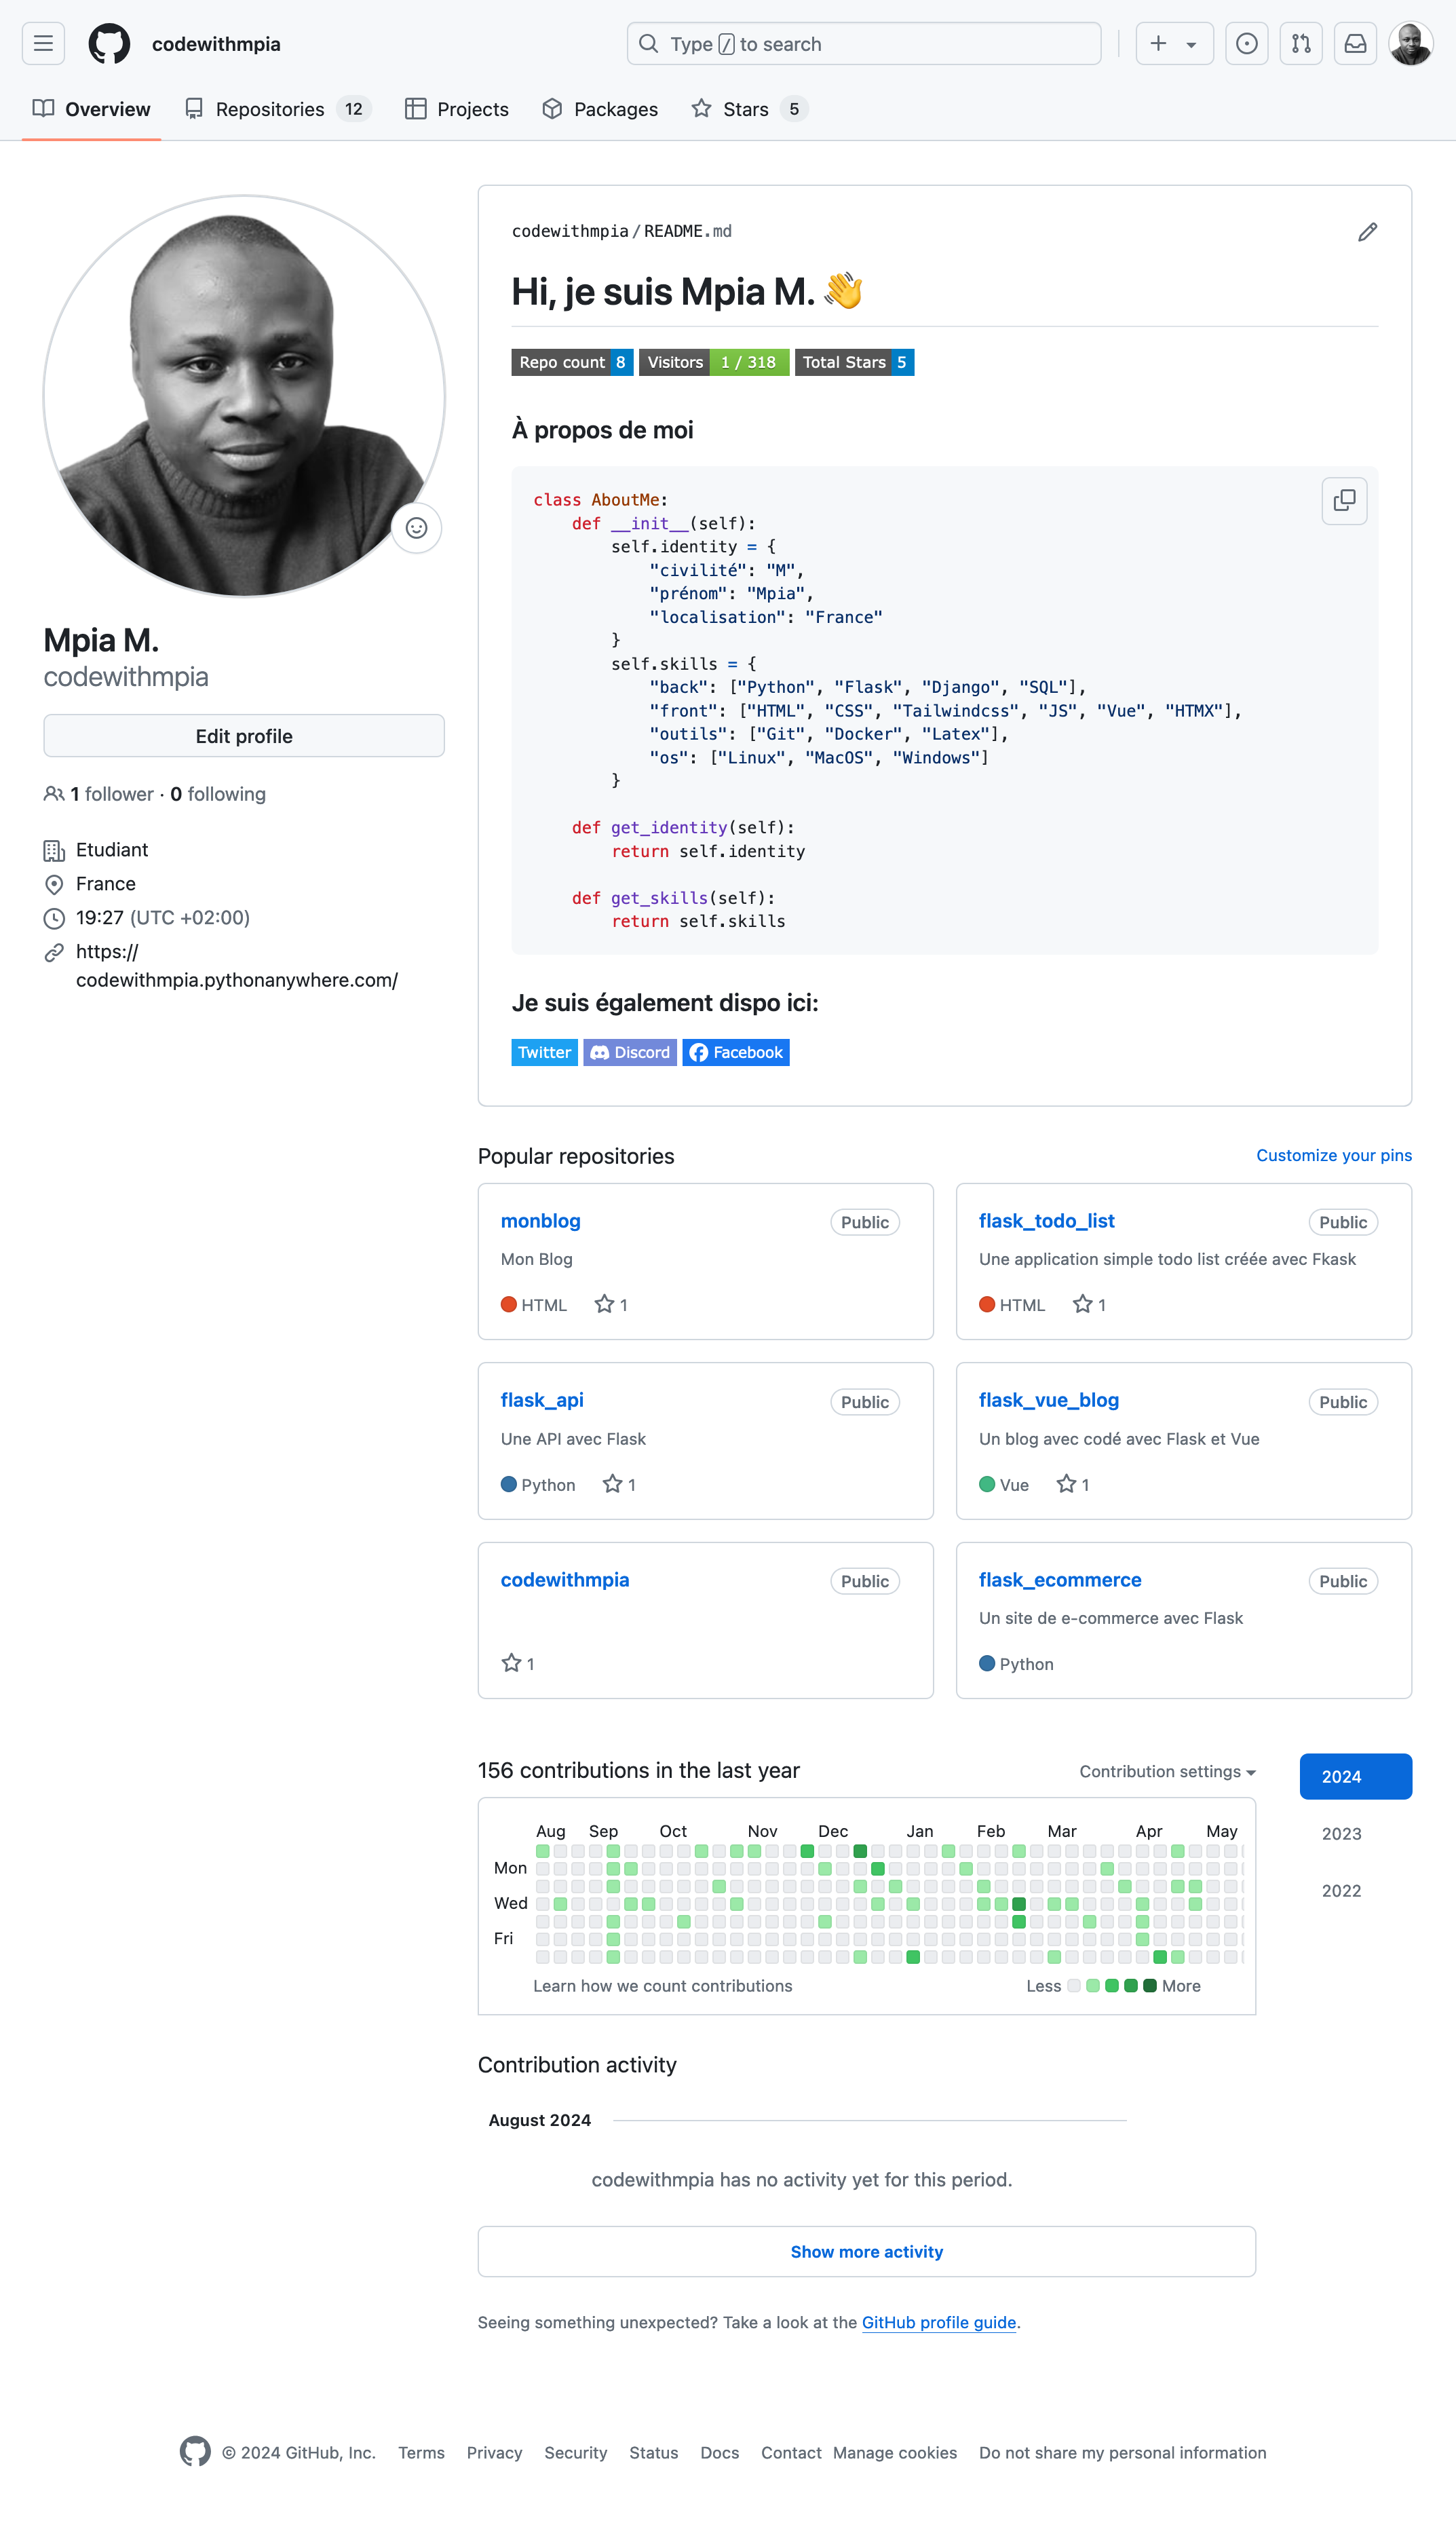
\includegraphics[width=0.8\textwidth]{TP-1/screen1.png}\\
            \includegraphics[width=0.9\textwidth]{TP-1/screen2.png}\\
            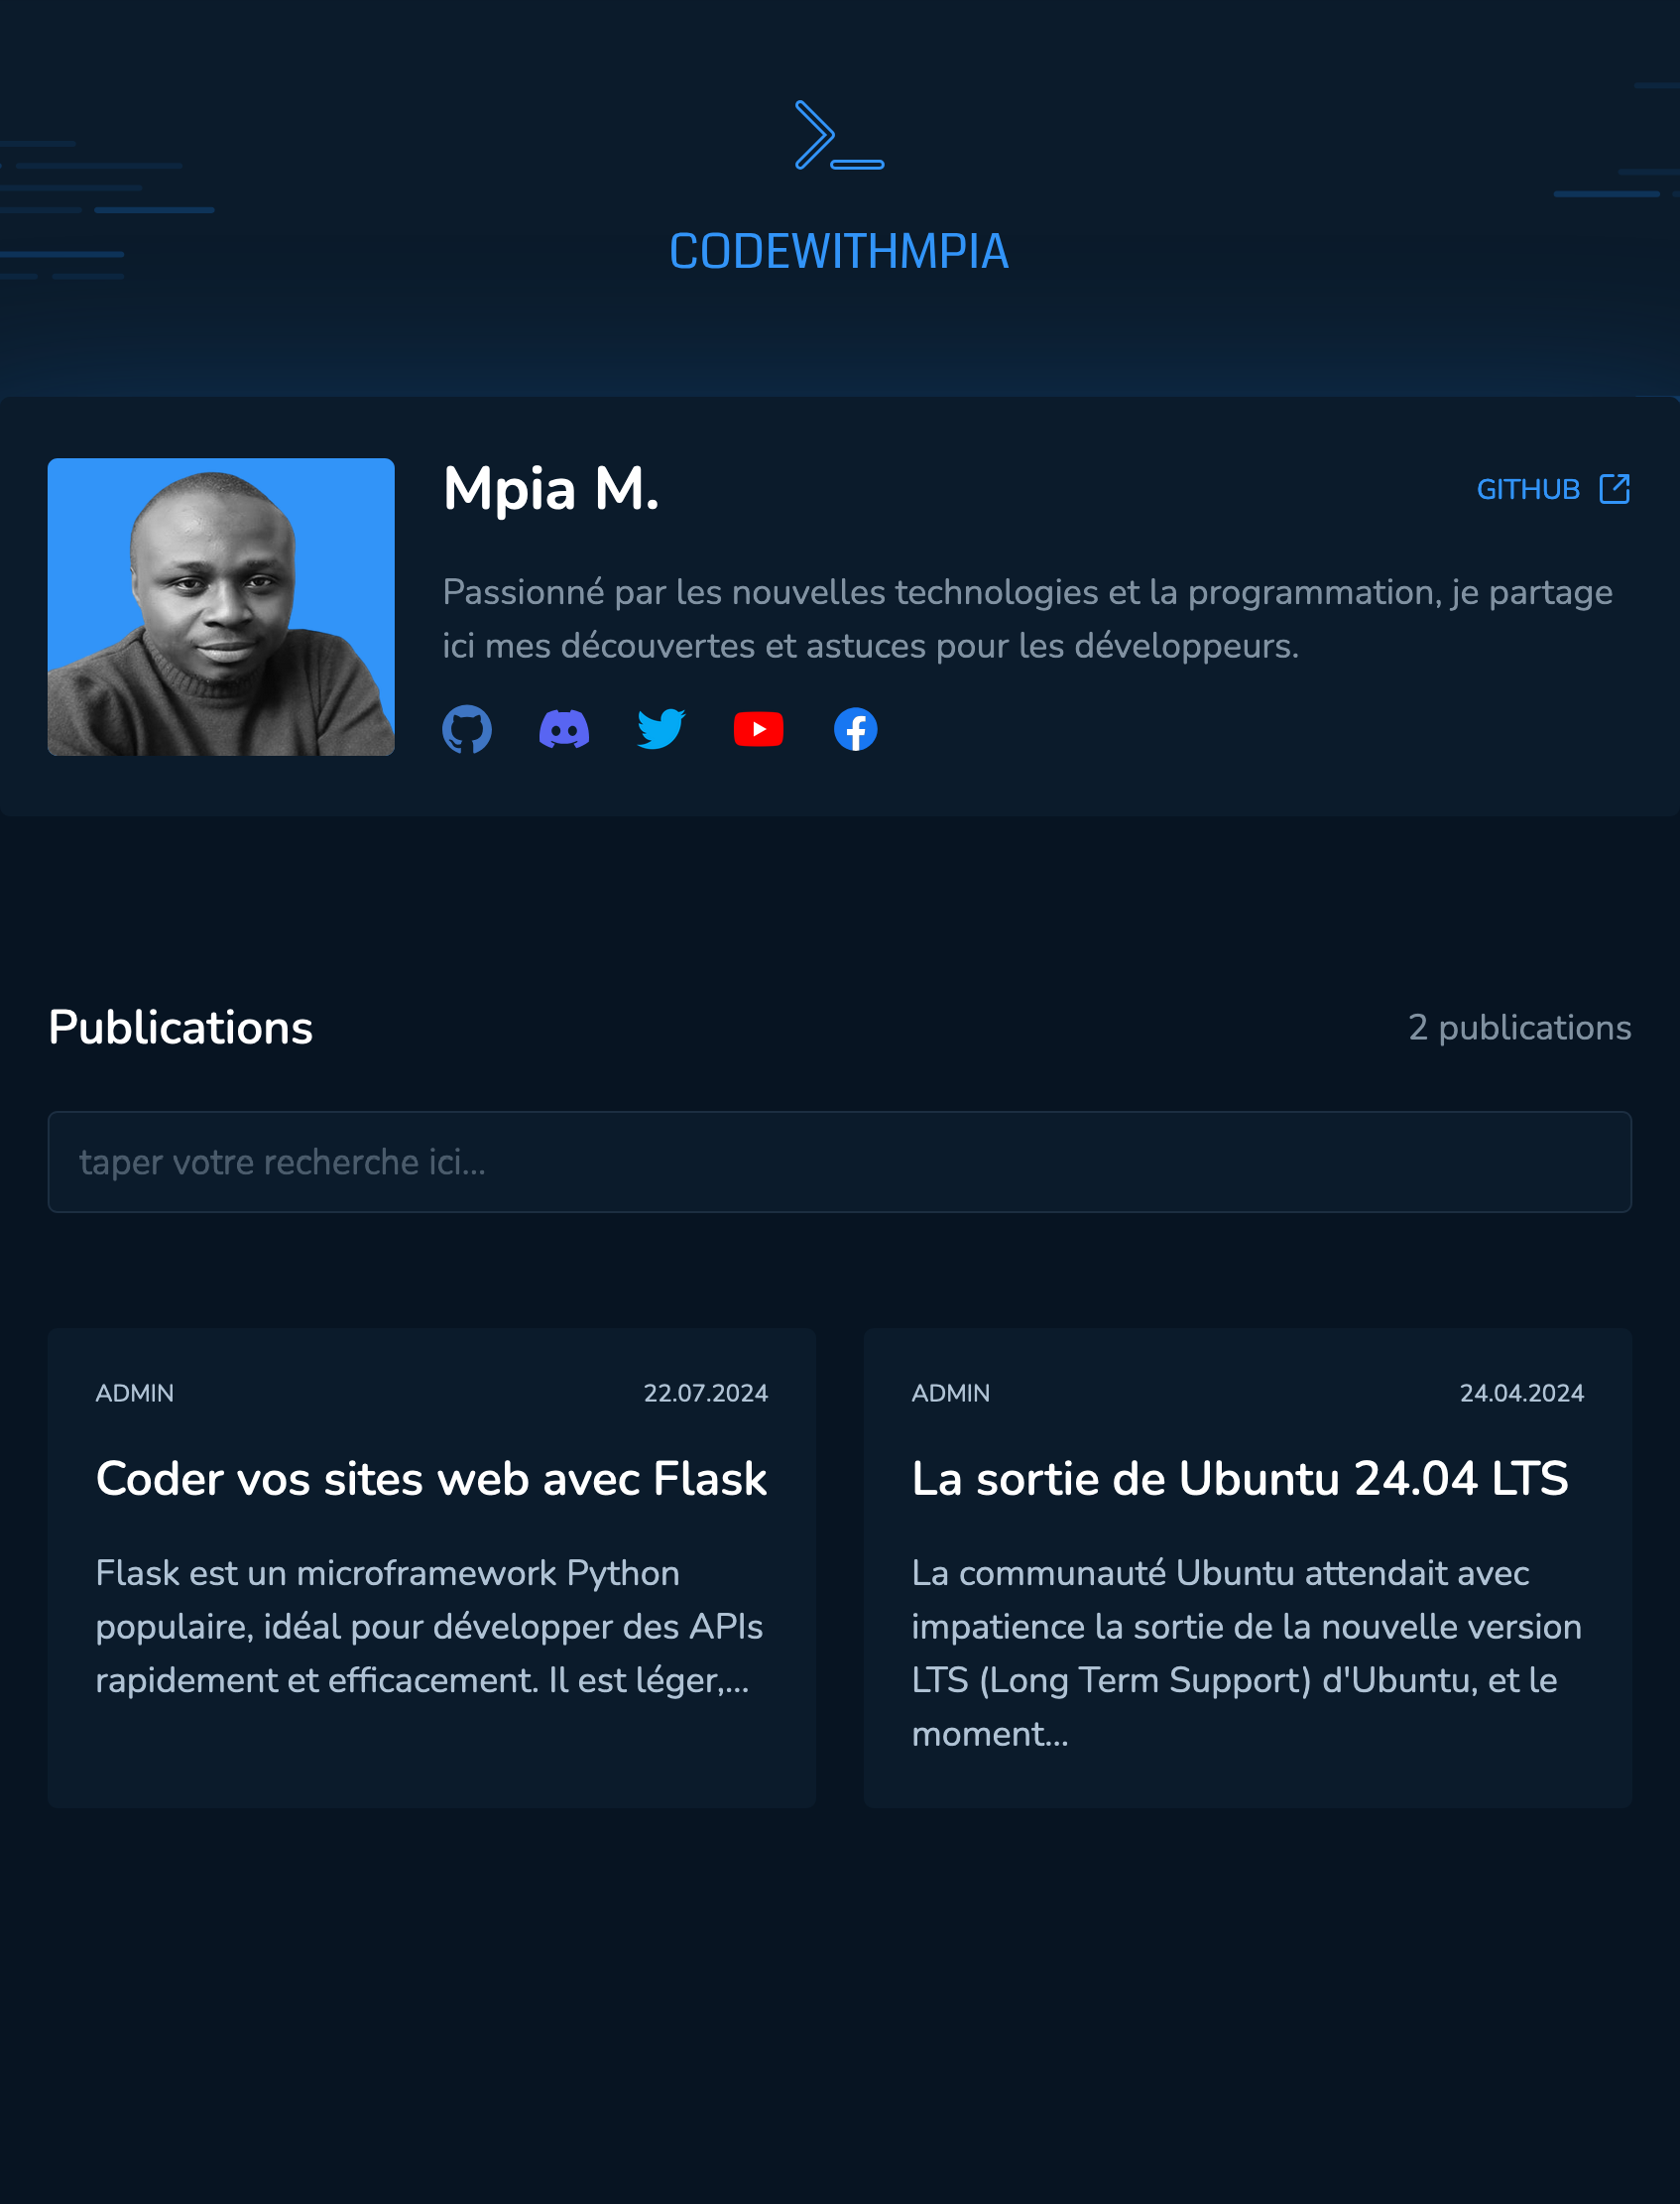
\includegraphics[width=0.9\textwidth]{TP-1/screen3.png}\\
            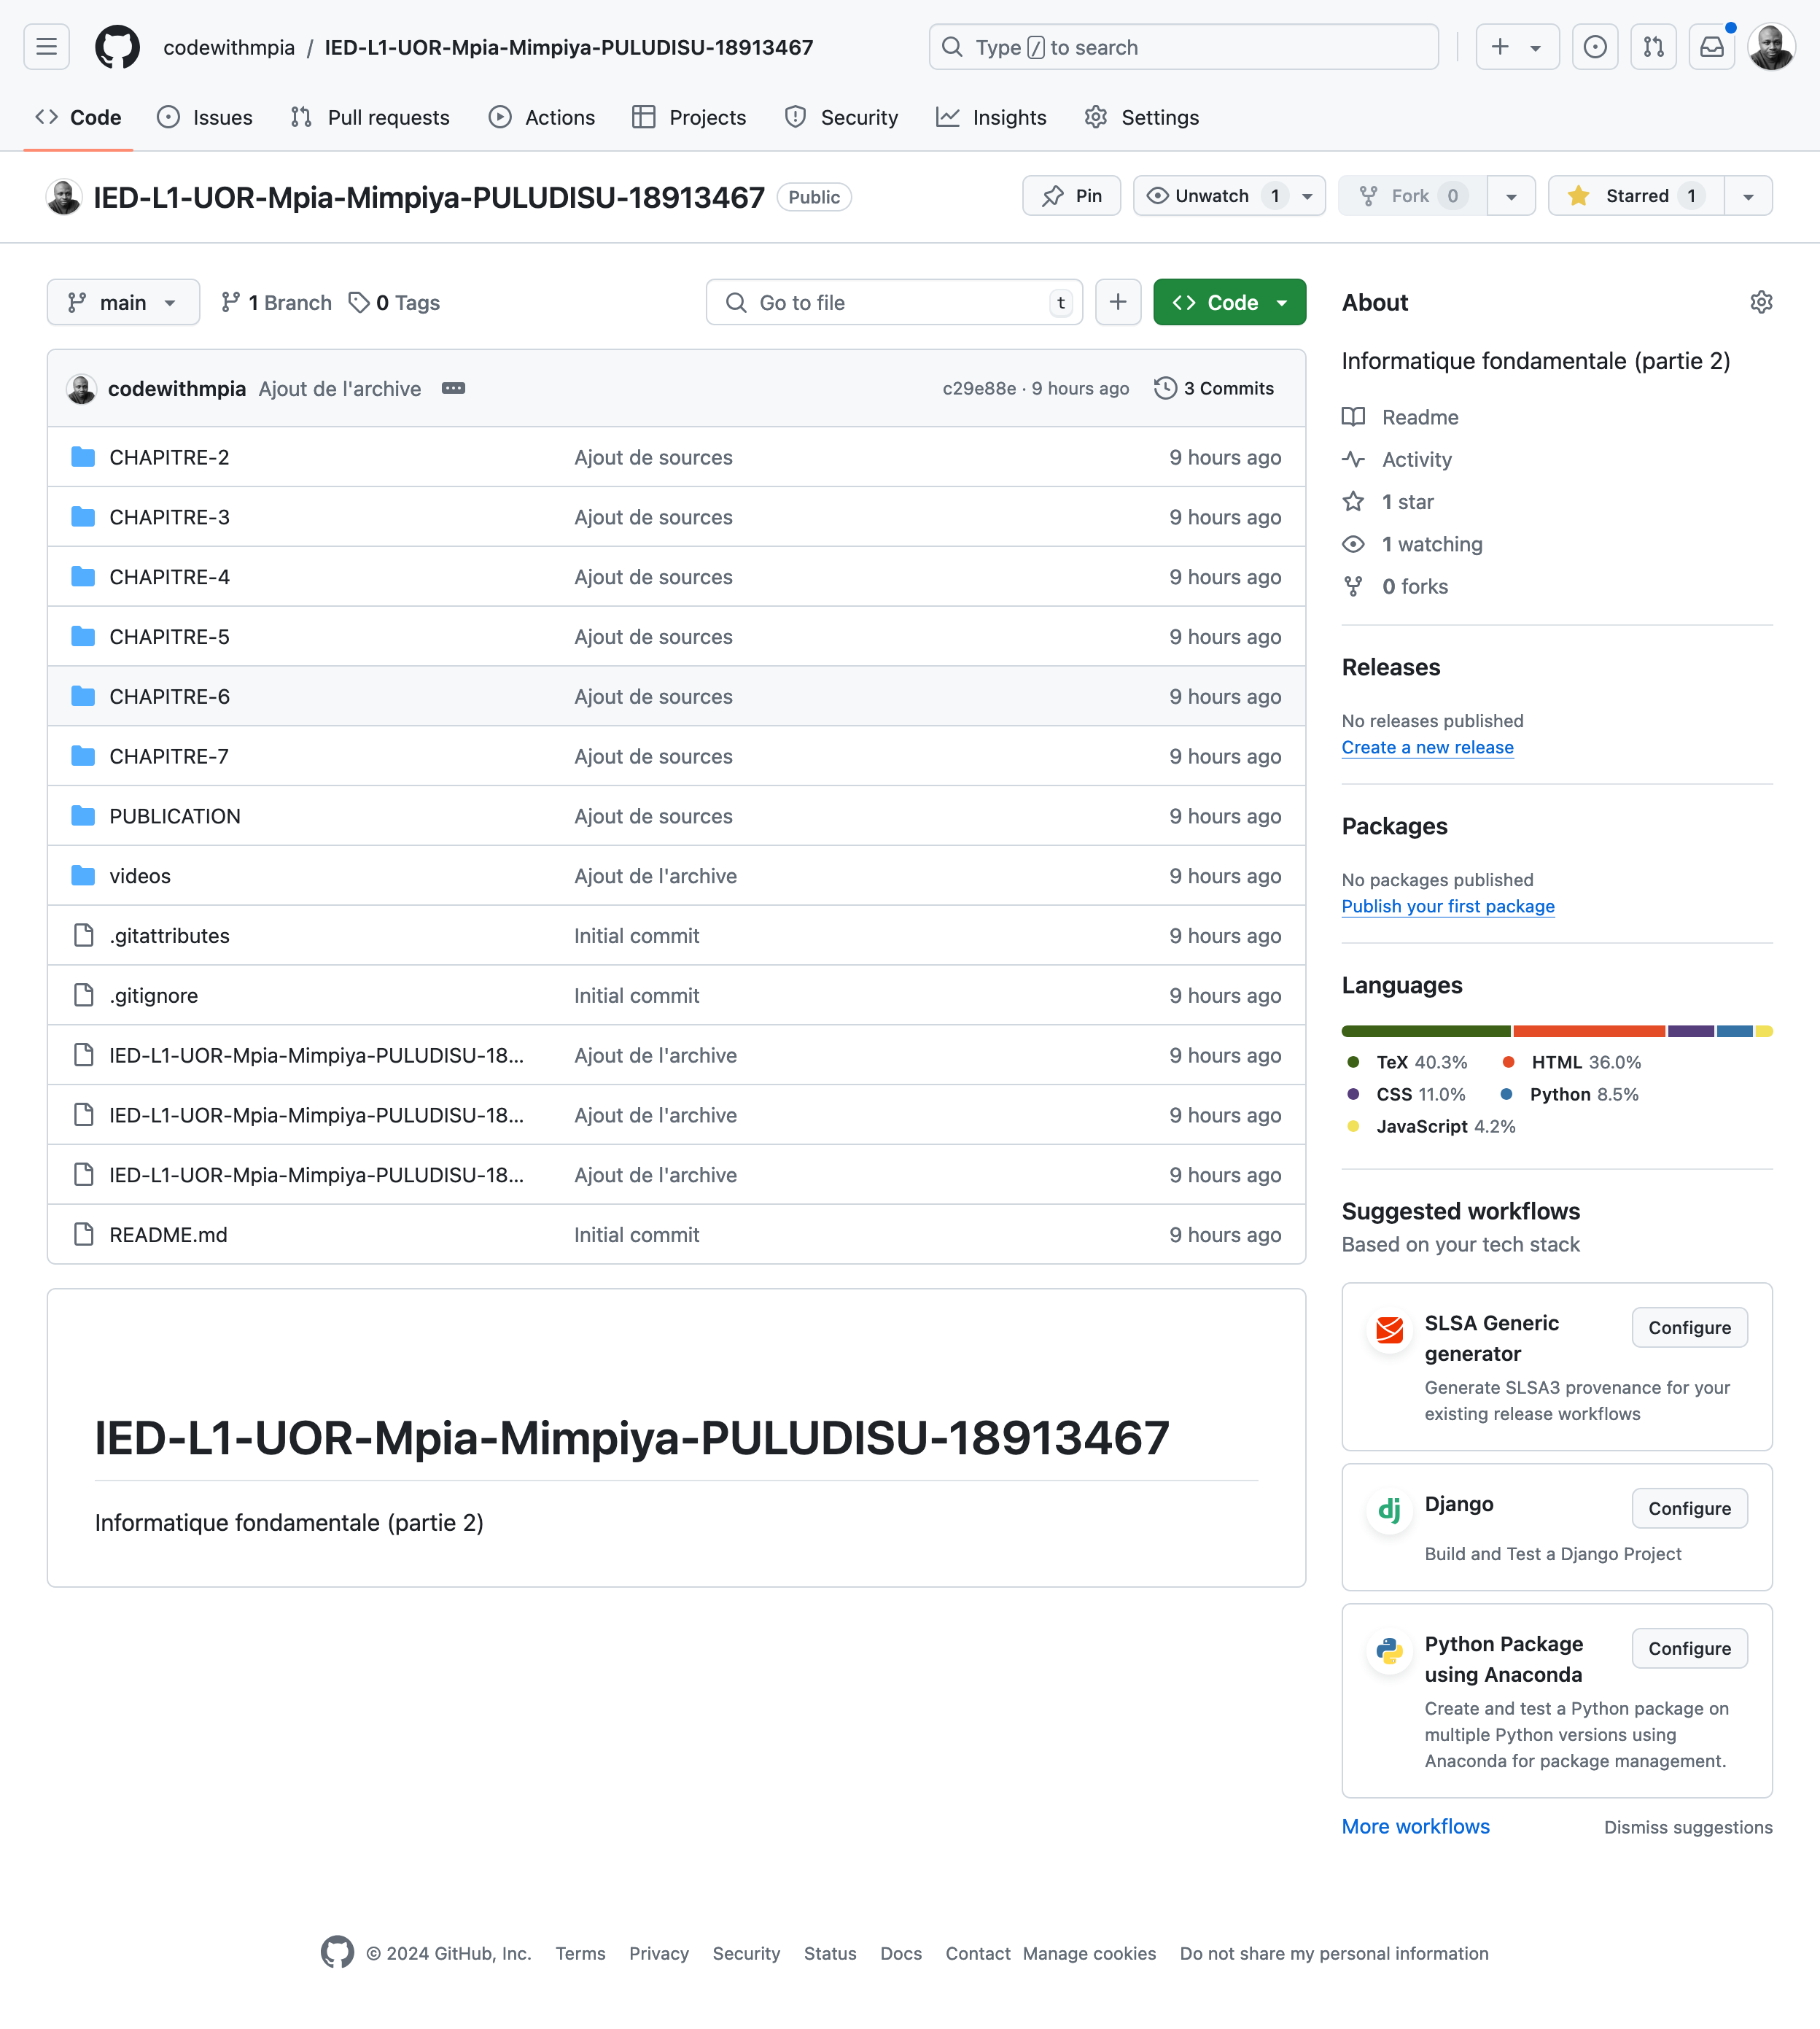
\includegraphics[width=0.9\textwidth]{TP-1/screen4.png}\\
            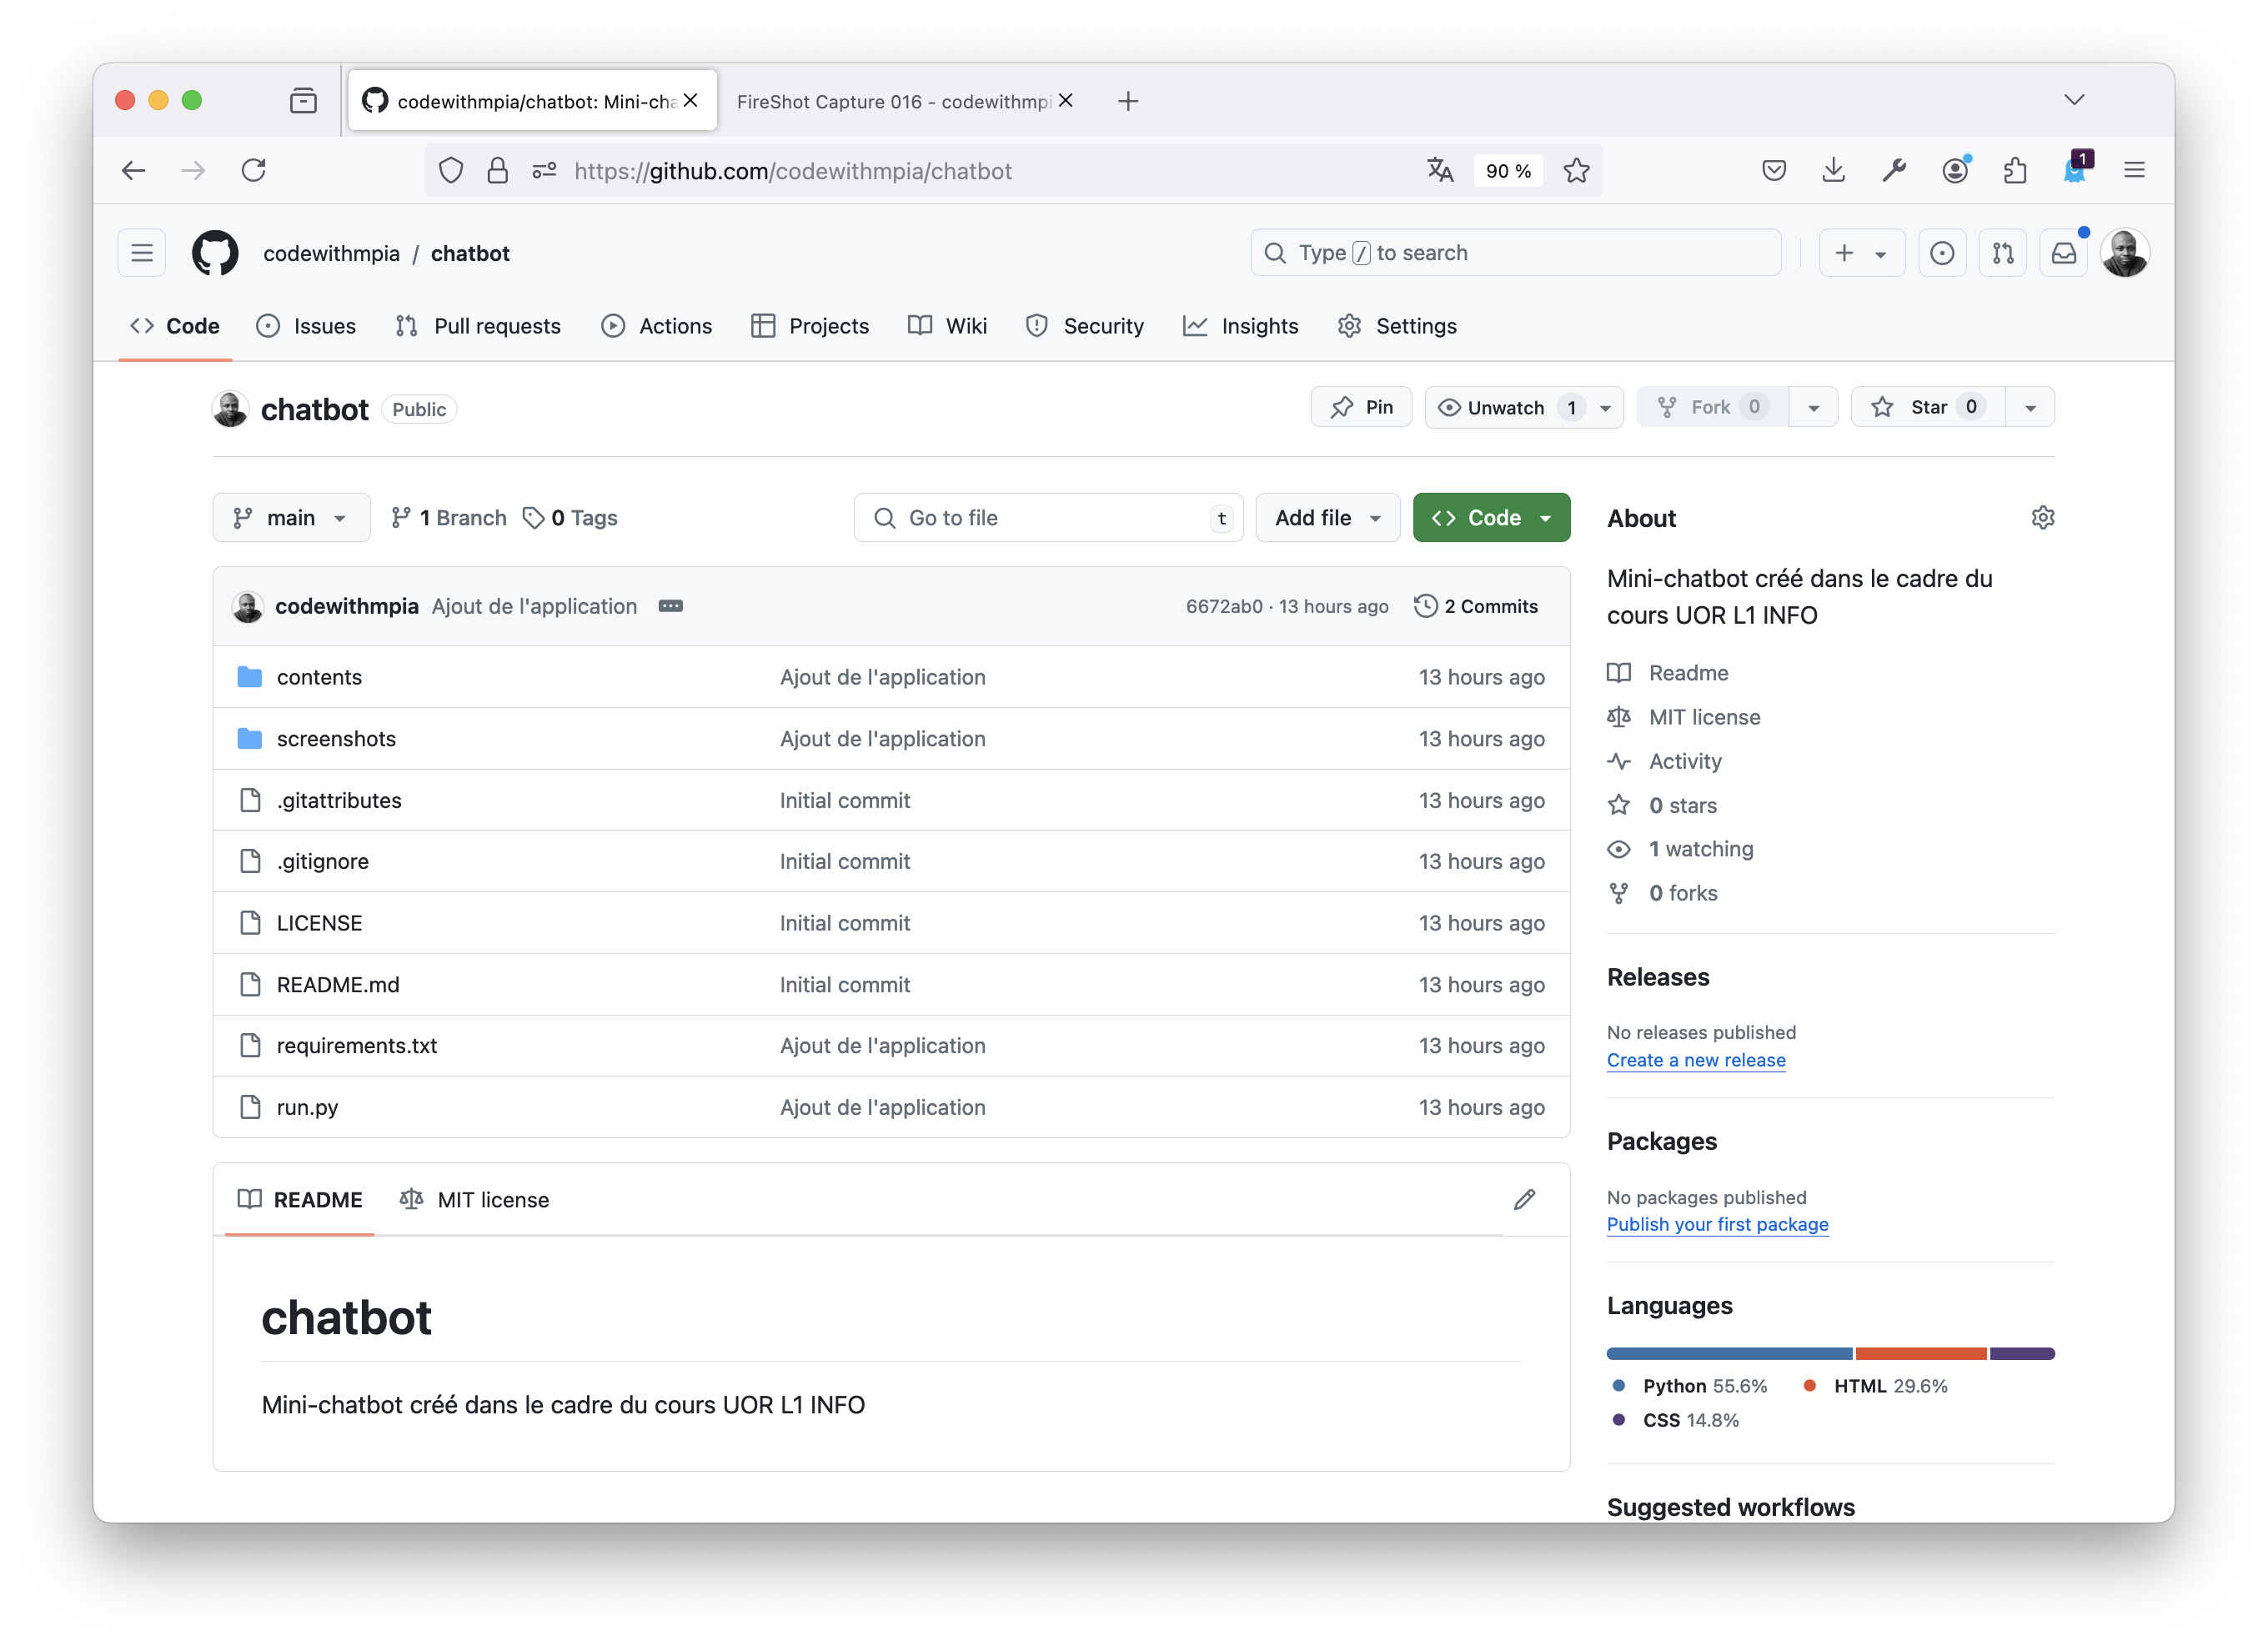
\includegraphics[width=0.9\textwidth]{TP-1/chatbot.png}\\
            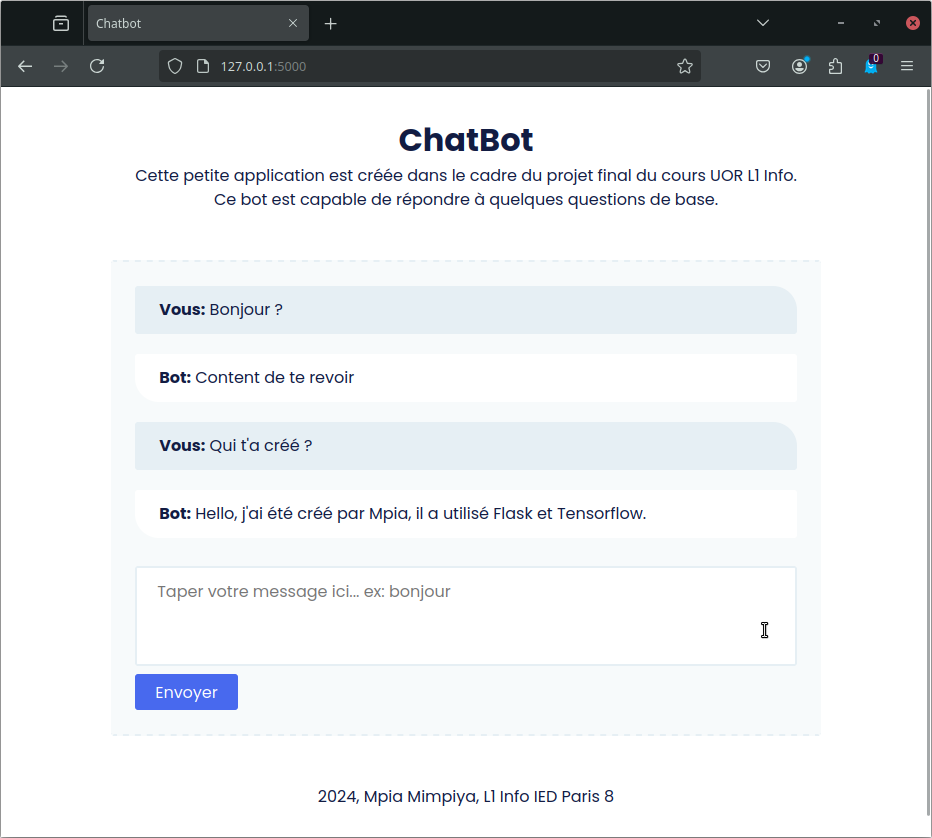
\includegraphics[width=0.9\textwidth]{TP-1/chatbot2.png}

            
    % TP 2
    \newpage
    \section{Deuxième partie: \\ TP 2 - Requêter à l’aide des API}
        \subsection{Attentu de la partie 2}
            \noindent Pour ce second chapitre, vous devez ajouter à votre PDF l'exercice 2.2.
            L'exercice 2.3 est pour un Bonus.

        \newpage
        \subsection{Exercice 2.2 (A Rendre)}
            \noindent \textit{En utilisant une ou plusieurs API de votre choix, comme par exemple, en choississant parmi 
            cette liste de liens (Google Books, Any API, Public API,API Gouv (Service Public) Open Data, Open Food Facts, ...), ou celles présentées dans ces notes ou autres :
            \begin{itemize}
                \item Réalisez à minima deux requêtes différentes (voire plus) afin de collecter de l’information que vous préciserez : (Quelle(s) infor- mation(s) ? Pour quoi faire ?, Comment ?, Quel(s) traitements ?, etc.).
                \item Produisez une ou plusieurs représentations graphiques des ré- sultats, à l’instar du cours, en n’oubliant pas d’indiquer vos motivations et d’en analyser les tendances et signaux remarquables.
                \item Pour les étudiant.e.s qui auraient déjà réalisé les TP(s) GIL, vous pouvez utiliser Tropes, Gephi ou encore des libraires de TAL (NLTK, TextBlob, SpaCy, GenSim, ...) , ou tout autre outil pour réali- ser une cartographie sémantique (graphe, nuage de mots, ...) ou une
                analyse de sentiments à l’aide de l’information collectée.
                \item  Les exemples ont été donnés en Python. Vous pouvez utiliser ce langage ou tout autre de votre choix. Renseignez bien les com- mandes et librairies utilisées et les directives de compilation si né-
                cessaire.
                \item N’oubliez pas, comme à l’habituée, d’expliquer votre méthodologie, d’insérer et de fournir les codes commentées avec métadon- nées descriptives (+ à joindre en archive attachée) et d’insérer des C.E(s) illustratives.
            \end{itemize}
            }

            \bigskip
            \noindent Pour réaliser ce projet, nous allons utiliser deux API différentes : Google Books API pour collecter des informations sur les livres et 
            Open Food Facts API pour collecter des informations sur les produits alimentaires. Nous allons ensuite analyser et visualiser les données collectées.

            \noindent Avant de se lancer, voici les modules python nécessaires:
                \lstinputlisting{TP-2/EXERCICE-2.2-A-RENDRE/requirements.txt}
            \noindent Bien entendu tous ces modules peuvent être installé en suivant les étapes suivantes:
                \begin{tcolorbox}[colback=lightgray!6, colframe=black, left=-40mm, right=5mm, top=2mm, bottom=-2mm, boxrule=0.1mm]
                    \begin{verbatim}
                        # créer un env virtuel
                        python -m venv venv ou python3 -m venv venv 
                        # activer le vitualenv
                        source venv/bin/activate 
                        # Installer les modules
                        pip install -r requirements.txt ou pip3 install requirements.txt
                    \end{verbatim}
                \end{tcolorbox}

            \newpage
            \begin{enumerate}
                \item \textbf{Collecte de données avec Google Books API}
                    \begin{itemize}
                        \item \underline{Objectif}: Collecter des informations sur les livres les plus populaires dans une catégorie spécifique (par exemple, "Science Fiction").
                        \item \underline{Méthologie}: 
                            \begin{itemize}
                                \item Utiliser l'API Google Books pour rechercher des livres dans la catégorie "Science Fiction".
                                \item Extraire des informations telles que le titre, l'auteur, la date de publication, et le nombre de pages.
                                \item Analyser les données pour identifier les tendances (par exemple, la longueur moyenne des livres).
                            \end{itemize}
                        \item \underline{Code Python}: 
                            \lstinputlisting{TP-2/EXERCICE-2.2-A-RENDRE/books.py}
                        \newpage
                        \item Visualisation (graphique):
                            \begin{figure}[ht]
                                \makebox[\textwidth][l]{
                                    \hspace{0.4cm}
                                    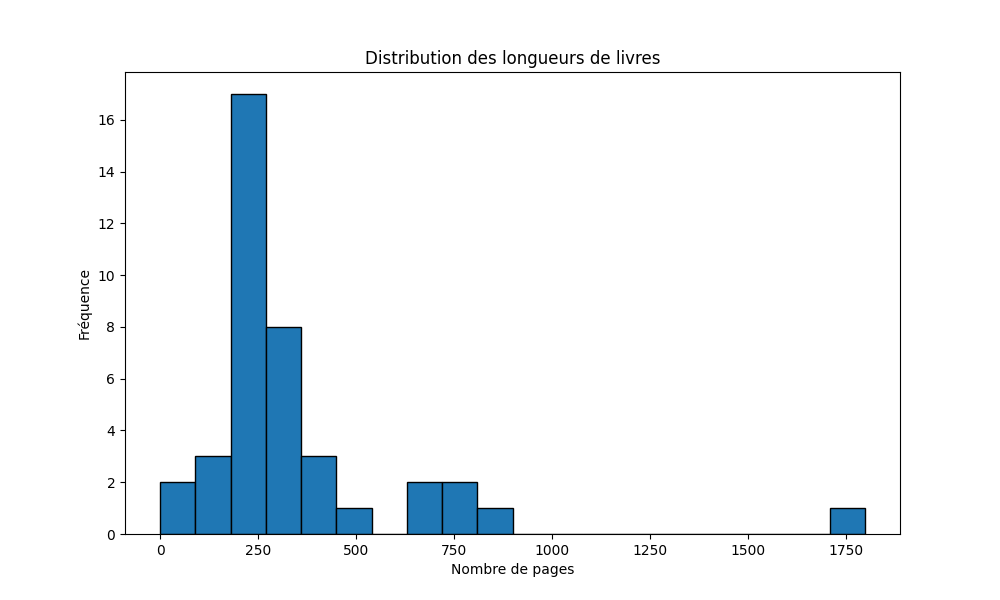
\includegraphics[width=0.8\textwidth]{TP-2/EXERCICE-2.2-A-RENDRE/screenshots/screen1.png}
                                }
                            \end{figure}
                    \end{itemize}

                \item \textbf{Collecte de données avec Open Food Facts API}
                    \begin{itemize}
                        \item \underline{Objectif}: Collecter des informations sur les produits alimentaires et analyser leur composition nutritionnelle.
                        \item \underline{Méthologie}:
                            \begin{itemize}
                                \item Utiliser l'API Open Food Facts pour rechercher des produits alimentaires.
                                \item Extraire des informations telles que le nom du produit, la marque, et les valeurs nutritionnelles (calories, sucres, graisses).
                                \item Analyser les données pour identifier les tendances (par exemple, la distribution des calories).
                            \end{itemize}
                        \item \underline{Code Python}: 
                            \lstinputlisting{TP-2/EXERCICE-2.2-A-RENDRE/foods.py}
                        \item Visualisation (graphique):
                            \begin{figure}[ht]
                                \makebox[\textwidth][l]{
                                    \hspace{0.4cm}
                                    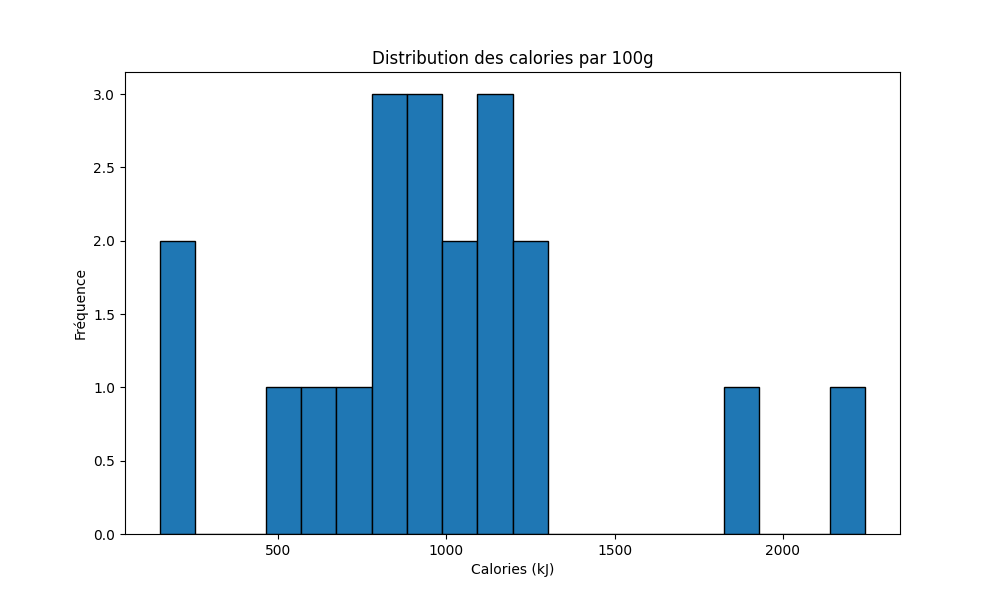
\includegraphics[width=0.8\textwidth]{TP-2/EXERCICE-2.2-A-RENDRE/screenshots/screen2.png}
                                }
                            \end{figure}
                    \end{itemize}
            \end{enumerate}

        \newpage  
        \subsection{Exercice 2.3 (Bonus)}
            \noindent \textit{A l'aide de la Librairie Python Selenium et avec API et la (les) requêtes de votre choix :
                \begin{itemize}
                    \item Concevez un programme qui collecte une dizaine d’adresses (URL) environ et qui génère dynamiquement les copies d’écran des sites web relativement à ces adresses.
                    \item Affichez ces copies d’écran avec les métadonnées de votre choix (adresse (URL), titre, ...) dans une page web à l’aide de Pyscript.
                    \item  Les étudiant.e.s qui auraient quelques difficultés avec Pyscript peuvent utiliser et rendre un Jupyter Notebook à la place. Soignez la présention et l’organisation de celui-ci en n’oubliant pas de le joindre à l’archive.
                    \item IL est également possible d’utilisr la librairie Pillow (ex PIL) pour afficher les images dans un GUI de votre choix...
                    \item Pensez à bien expliquer vos choix, vos méthodes et à bien citer les sources utilisées.
                \end{itemize}
            }
            
            \bigskip
            \noindent Pour réaliser ce projet, nous allons suivre les étapes suivantes :
            
            \begin{enumerate}
                \item \underline{Collecte des adresses (URL)}: Nous allons utiliser une liste prédéfinie d'URL pour simplifier le processus.
                \item \underline{Génération des copies d'écran}: Nous allons utiliser Selenium pour capturer les copies d'écran des sites web.
                \item \underline{Affichage des copies d'écran avec les métadonnées}: Nous allons utiliser Pyscript pour créer une page web qui affiche les copies d'écran avec les métadonnées.
            \end{enumerate}

            \bigskip
            \noindent Les modules suivants sont nécessaires:
            \lstinputlisting{TP-2/EXERCICE-2.3-BONUS/requirements.txt}

            \noindent Ces modules peuvent tous être installés de cette façon:
            \begin{tcolorbox}[colback=lightgray!6, colframe=black, left=-40mm, right=5mm, top=2mm, bottom=-2mm, boxrule=0.1mm]
                \begin{verbatim}
                    # créer un env virtuel
                    python -m venv venv ou python3 -m venv venv 
                    # activer le vitualenv
                    source venv/bin/activate 
                    # Installer les modules
                    pip install -r requirements.txt ou pip3 install requirements.txt
                \end{verbatim}
            \end{tcolorbox}

            \noindent 

            \noindent Voici le code Python réalisant cette tâche: 
                \lstinputlisting{TP-2/EXERCICE-2.3-BONUS/main.py}
            
            \noindent Une fois tous les modules instalés, vous exécuter le code contenu dans \textbf{main.py} pour faire de captures de sites web avec Selenium:
                \begin{tcolorbox}[colback=lightgray!6, colframe=black, left=-40mm, right=5mm, top=2mm, bottom=-2mm, boxrule=0.1mm]
                    \begin{verbatim}
                        python main.py ou python3 main.py
                    \end{verbatim}
                \end{tcolorbox}
            
            \noindent Maintenant que toutes les captures de sites web sont faites et sauvegardées dans le dossier nommé
            \textbf{srcreenshots/}, nous pouvons ouvrir le fichier \textbf{index.html} avec le navigateur de notre choix, comme google-chrome ou 
            firefox pour voir les captures de sites web sous forme d'une galéries d'images. 
            J'ai mis ces images dans des liens vers le site web correspondant. 
            
            \newpage 
            \noindent Voici le contenu du fichier \textbf{index.html}: 
            \lstinputlisting{TP-2/EXERCICE-2.3-BONUS/index.html}
            
            \newpage
            \noindent Voici à quoi ressemble cette petite page web:

            \begin{figure}[ht]
                \makebox[\textwidth][l]{
                    \hspace{0.4cm}
                    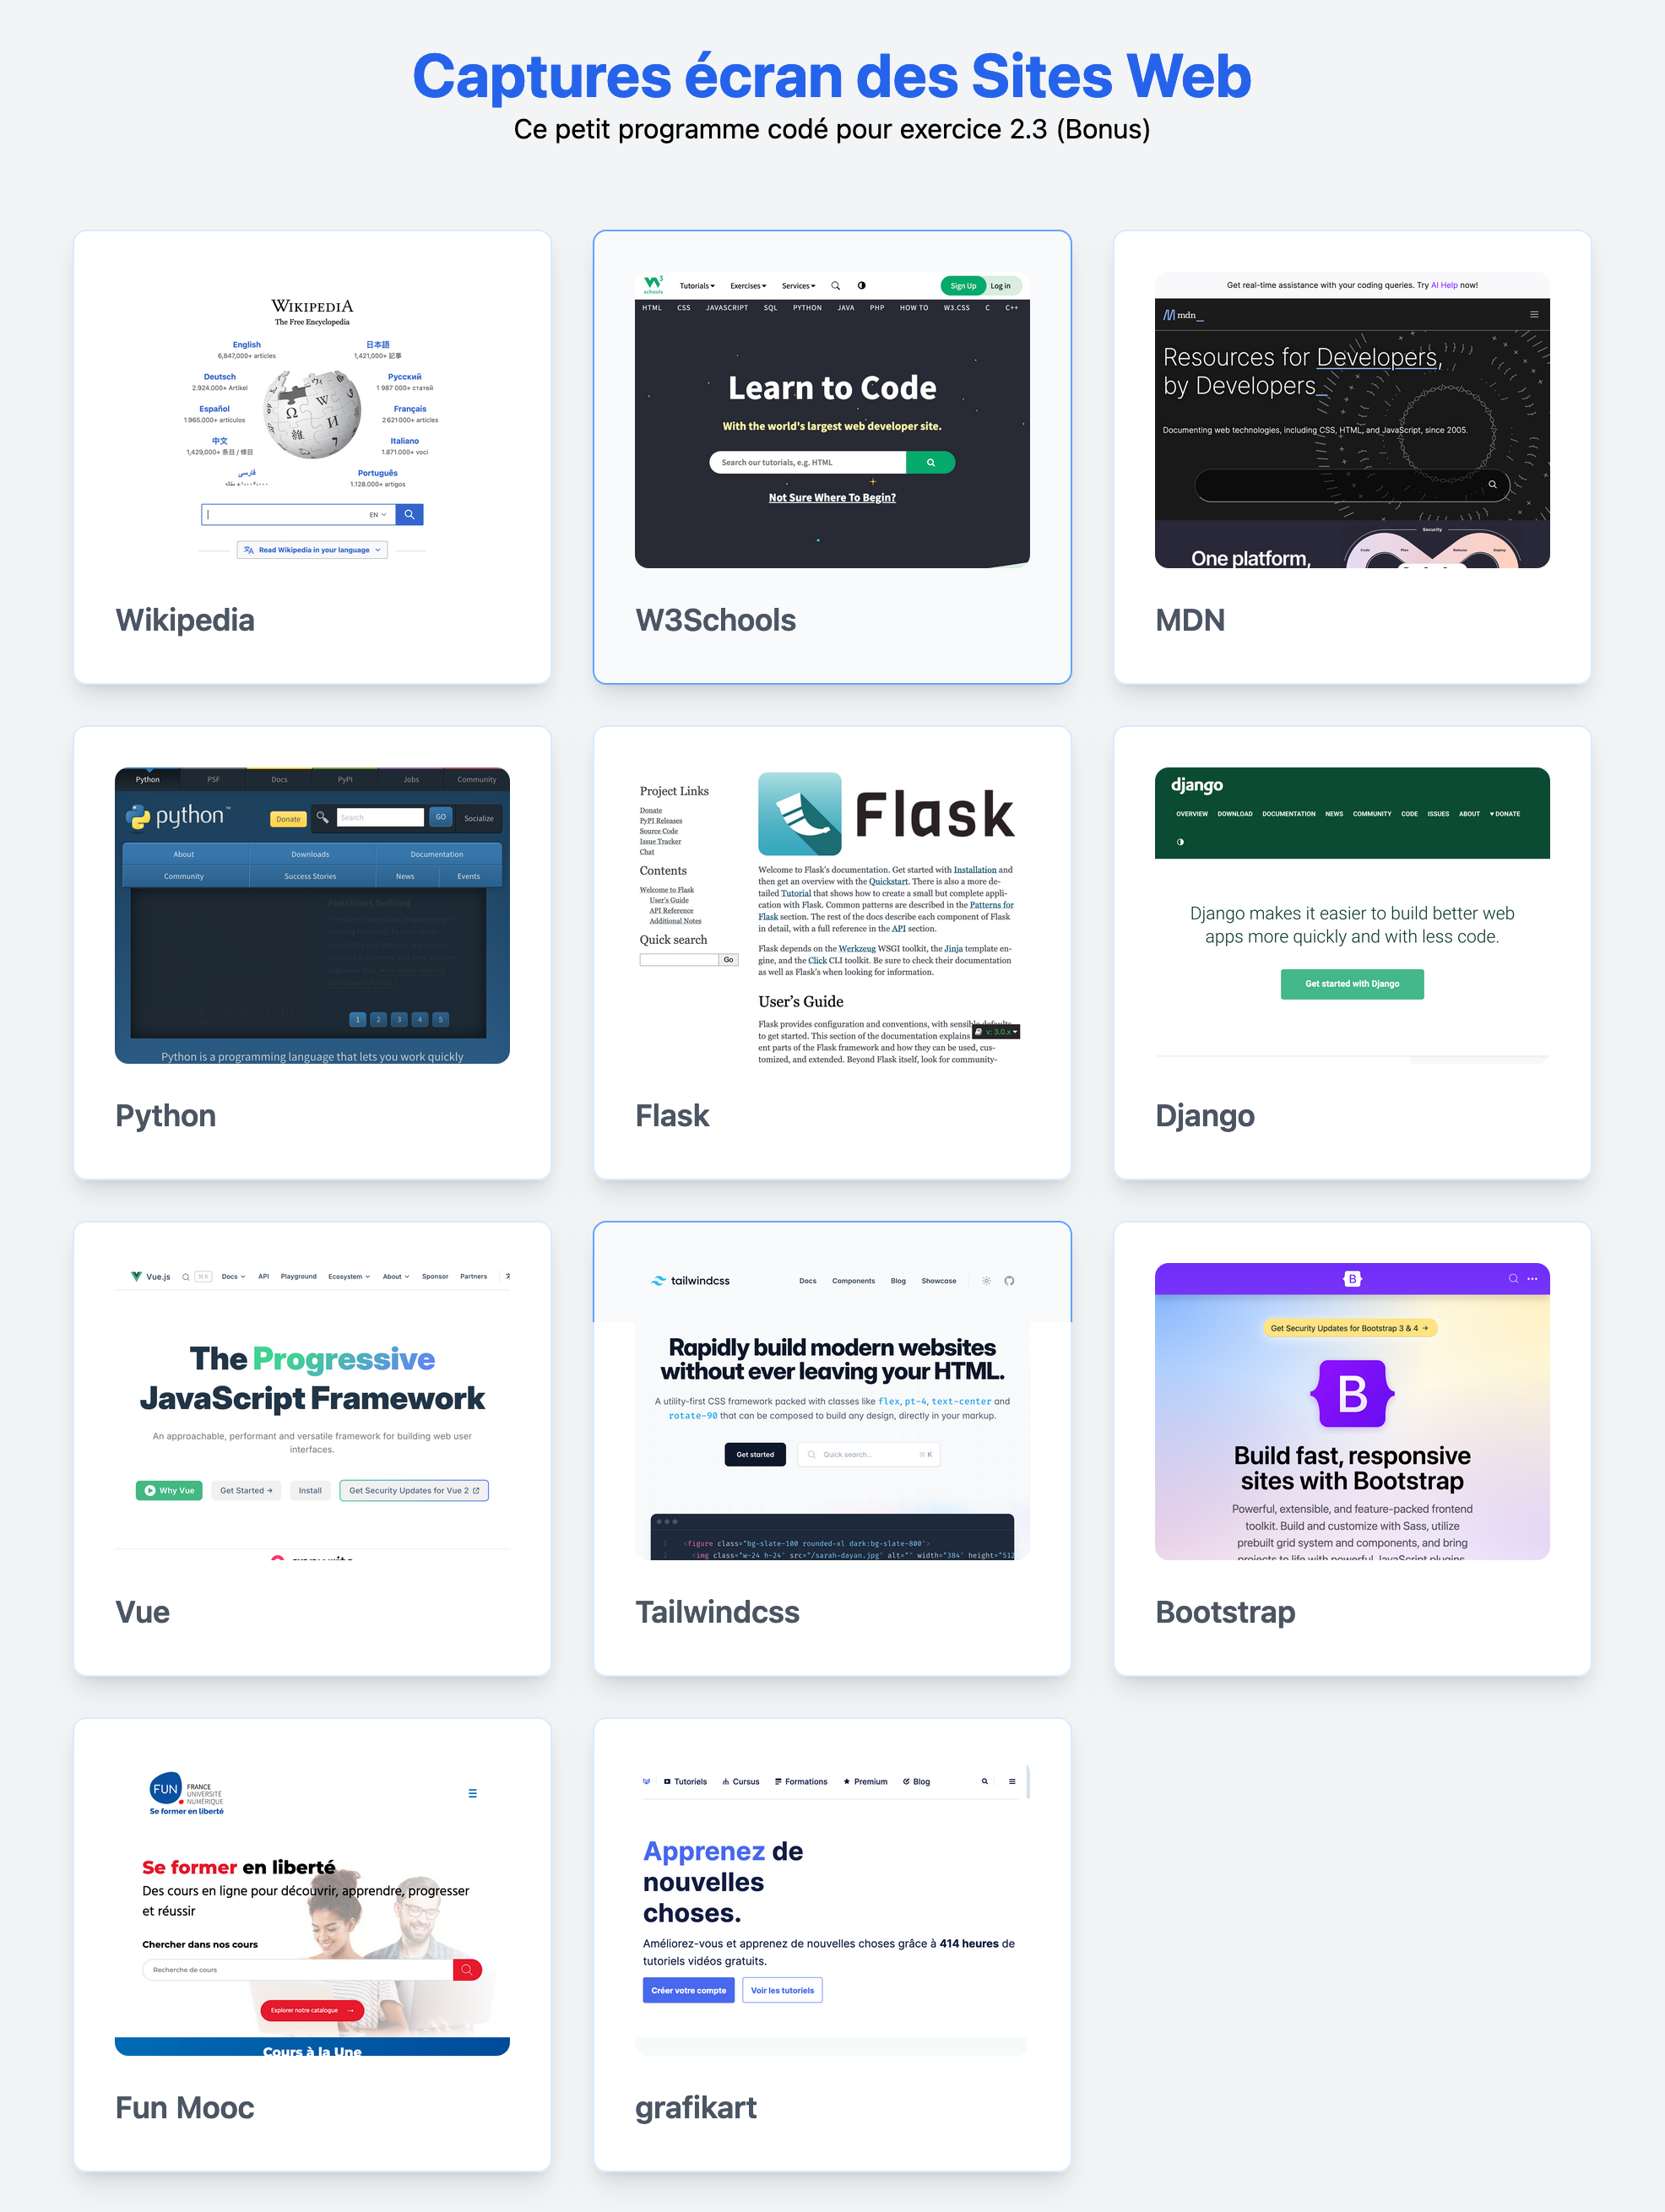
\includegraphics[width=0.6\textwidth]{TP-2/EXERCICE-2.3-BONUS/screen.png}
                }
            \end{figure}
            
            \begin{tcolorbox}[colback=lightgray!6, colframe=black, left=5mm, right=5mm, top=2mm, bottom=2mm, boxrule=0.1mm]
                La collecte et le traitement de données via une API, comme illustré dans ces deux exemples, montrent la puissance et la flexibilité des outils modernes de développement. En utilisant la bibliothèque requests pour interagir avec l'API Open Food Facts, l'API de Google Books, nous avons pu récupérer des informations sur des produits alimentaires spécifiques, des livres sur la Science Fiction.\\

                La conversion des données récupérées en un DataFrame Pandas a permis une manipulation et une analyse efficaces. Nous avons pu extraire et calculer des statistiques pertinentes, telles que les moyennes des calories, des sucres et des graisses par 100g. Cette analyse a été facilitée par la conversion des valeurs en types numériques et la gestion des valeurs manquantes.\\

                La visualisation des données avec Matplotlib a offert une représentation claire de la distribution des calories par exemple, permettant une meilleure compréhension des tendances et des variations dans les produits alimentaires.\\

                En résumé, ce processus démontre comment l'intégration de différentes bibliothèques Python (requests, pandas, matplotlib) peut être utilisée pour automatiser la collecte, le traitement et la visualisation de données, offrant ainsi des insights précieux et actionnables.
            \end{tcolorbox}
        
    % TP 3
    \newpage
    \section{Troisième partie \\ TP 3 - Créer sa Propre API}
        \subsection{Attentus de la partie 3}
            \noindent Pour ce troisième chapitre, l'exercice 3.1 est assez facile à réaliser. L'exercice
            3.2 qui explore la reconnaissance faciale est pour un Bonus bien mérité.

        \newpage
        \subsection{Exercice 3.1 (A Rendre)}
            \noindent \textit{En vous inspirant du code-source contenu dans la section "Squelette d’Application à Adapter" :
            \begin{itemize}
                \item Développez votre propre application FastAPI dans la thématique de votre choix, en y insérant un jeu de données à consulter et à partager collaborativement.
            \end{itemize}
            }
            \bigskip
            \noindent Pour répondre à la question de création d'une application FastAPI qui permet de consulter et de partager collaborativement un jeu de données, nous allons suivre les étapes suivantes :
                \begin{enumerate}
                    \item \textbf{Définir le jeu de données}: \\Nous allons créer un jeu de données de publications avec des commentaires associés. Chaque publication aura un titre, un résumé, un contenu, un nombre de vues, une image, une date de création et un statut de publication. Chaque commentaire aura un auteur, un message, une date de création et un identifiant de publication.
                    \item \textbf{Configurer la base de données}:\\ Nous allons utiliser SQLite pour stocker les données. Nous créerons deux tables : posts pour les publications et comments pour les commentaires.
                    \item \textbf{Créer les modèles de données}:\\ Nous définirons les modèles Pydantic pour les publications et les commentaires. Ces modèles seront utilisés pour valider les données entrantes et sortantes.
                    \item \textbf{Développer les endpoints de l'API}: Nous créerons des endpoints pour lister, créer, mettre à jour, supprimer des publications et créer des commentaires.
                        \begin{itemize}
                            \item \underline{GET /api/posts/} : Récupérer la liste des publications publiées.
                            \item \texttt{GET /api/posts/\{post\_id\}/} : Récupérer les détails d'une publication spécifique.
                            \item \underline{POST /api/posts/create/} : Créer une nouvelle publication.
                            \item \underline{DELETE /api/posts/\{post\_id\}/} : Supprimer une publication.
                            \item \underline{POST /api/comments/create/}: Créer un nouveau commentaire pour une publication.
                        \end{itemize}
                    \item \textbf{Tester l'application}: \\ Nous utiliserons l'interface interactive de FastAPI (/docs) pour tester les endpoints. Nous pouvons également utiliser des outils comme HTTPie, Insomnia pour envoyer des requêtes HTTP et tester les endpoints.
                \end{enumerate}

                \noindent Voici les modules nécessaires à la réalisation de notre api, qui je le rappelle doit me mettre de servir 
                les aricles de blog de mon future site web: 

                \lstinputlisting{TP-3/EXERCICE-3.1-A-RENDRE/requirements.txt}

                \noindent Commençons par créeer un environnement virtuel et installons les différents modules:
                    \begin{tcolorbox}[colback=lightgray!6, colframe=black, left=-40mm, right=5mm, top=2mm, bottom=-2mm, boxrule=0.1mm]
                        \begin{verbatim}
                            # créer un env virtuel
                            python -m venv venv ou python3 -m venv venv 
                            # activer le vitualenv
                            source venv/bin/activate 
                            # Installer les modules
                            pip install -r requirements.txt ou pip3 install requirements.txt
                        \end{verbatim}
                    \end{tcolorbox}
            \newpage
            \noindent Voici le code complet de cette API: 

            \lstinputlisting{TP-3/EXERCICE-3.1-A-RENDRE/main.py}
            
            \newpage
            \noindent Voici quelques captures d'écran: 
            \begin{figure}[ht]
                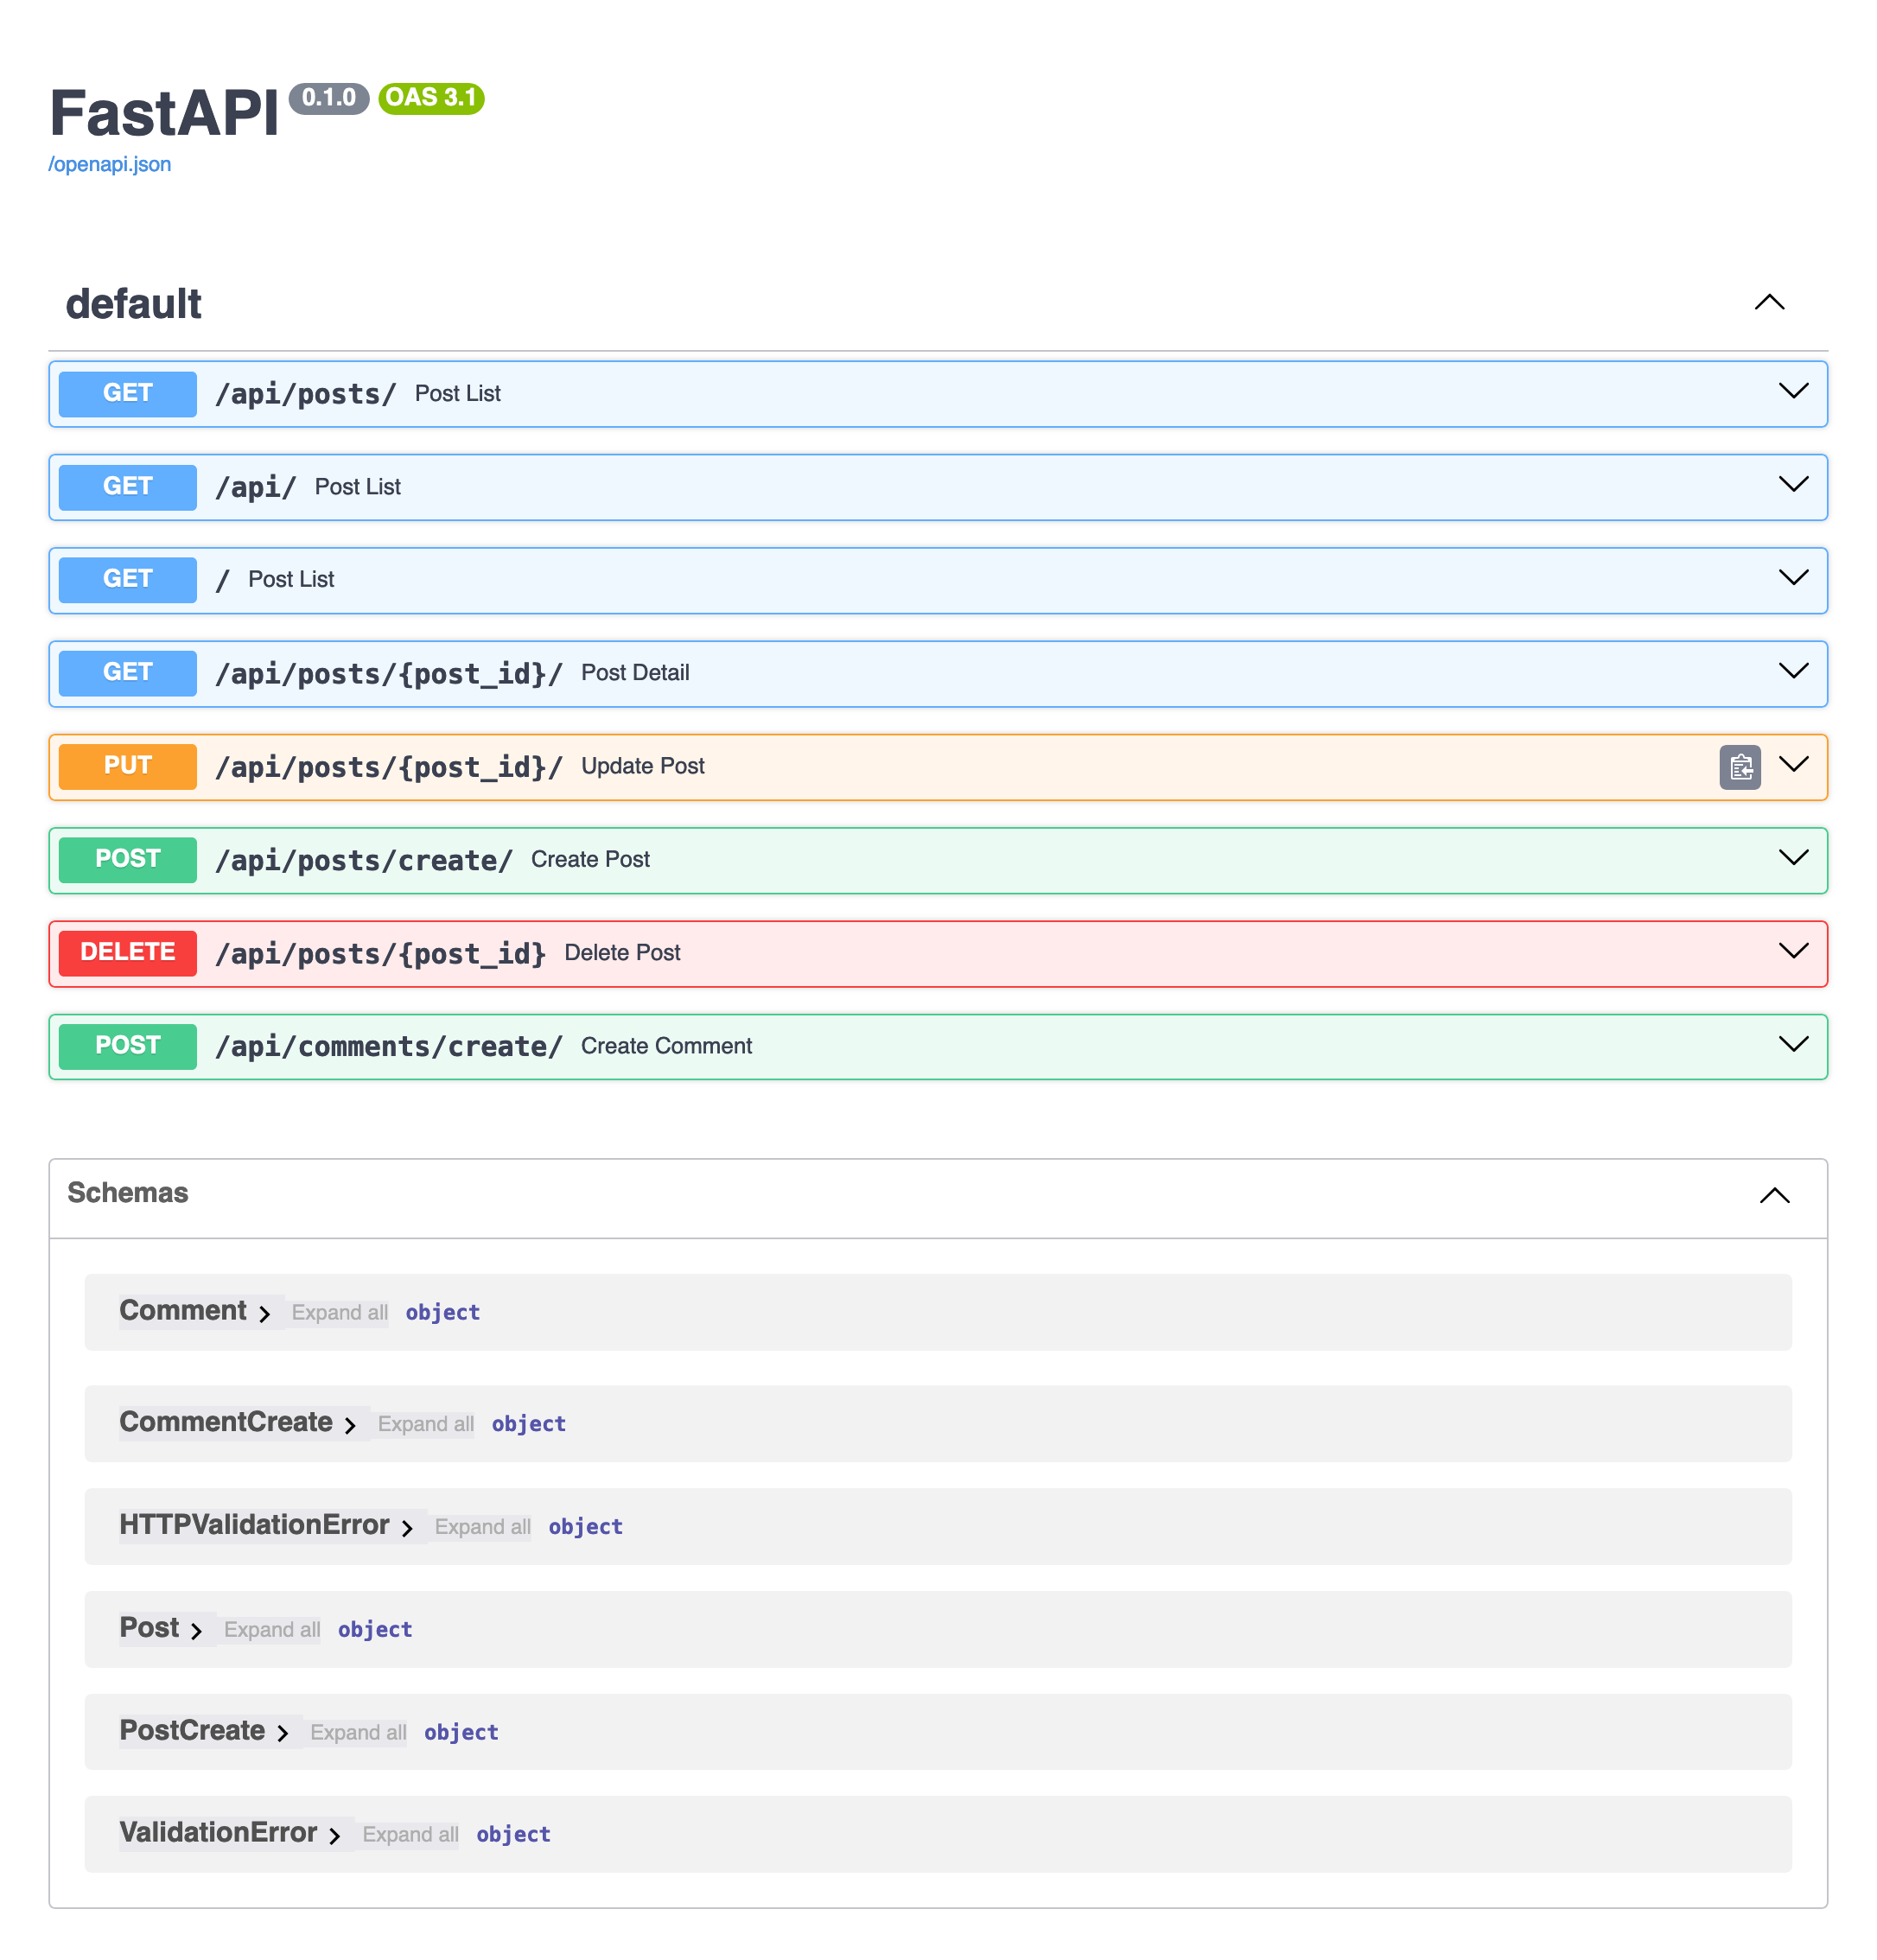
\includegraphics[width=0.8\textwidth]{TP-3/EXERCICE-3.1-A-RENDRE/screenshots/doc.png}
            \end{figure}

            \newpage
            \begin{figure}[ht]
                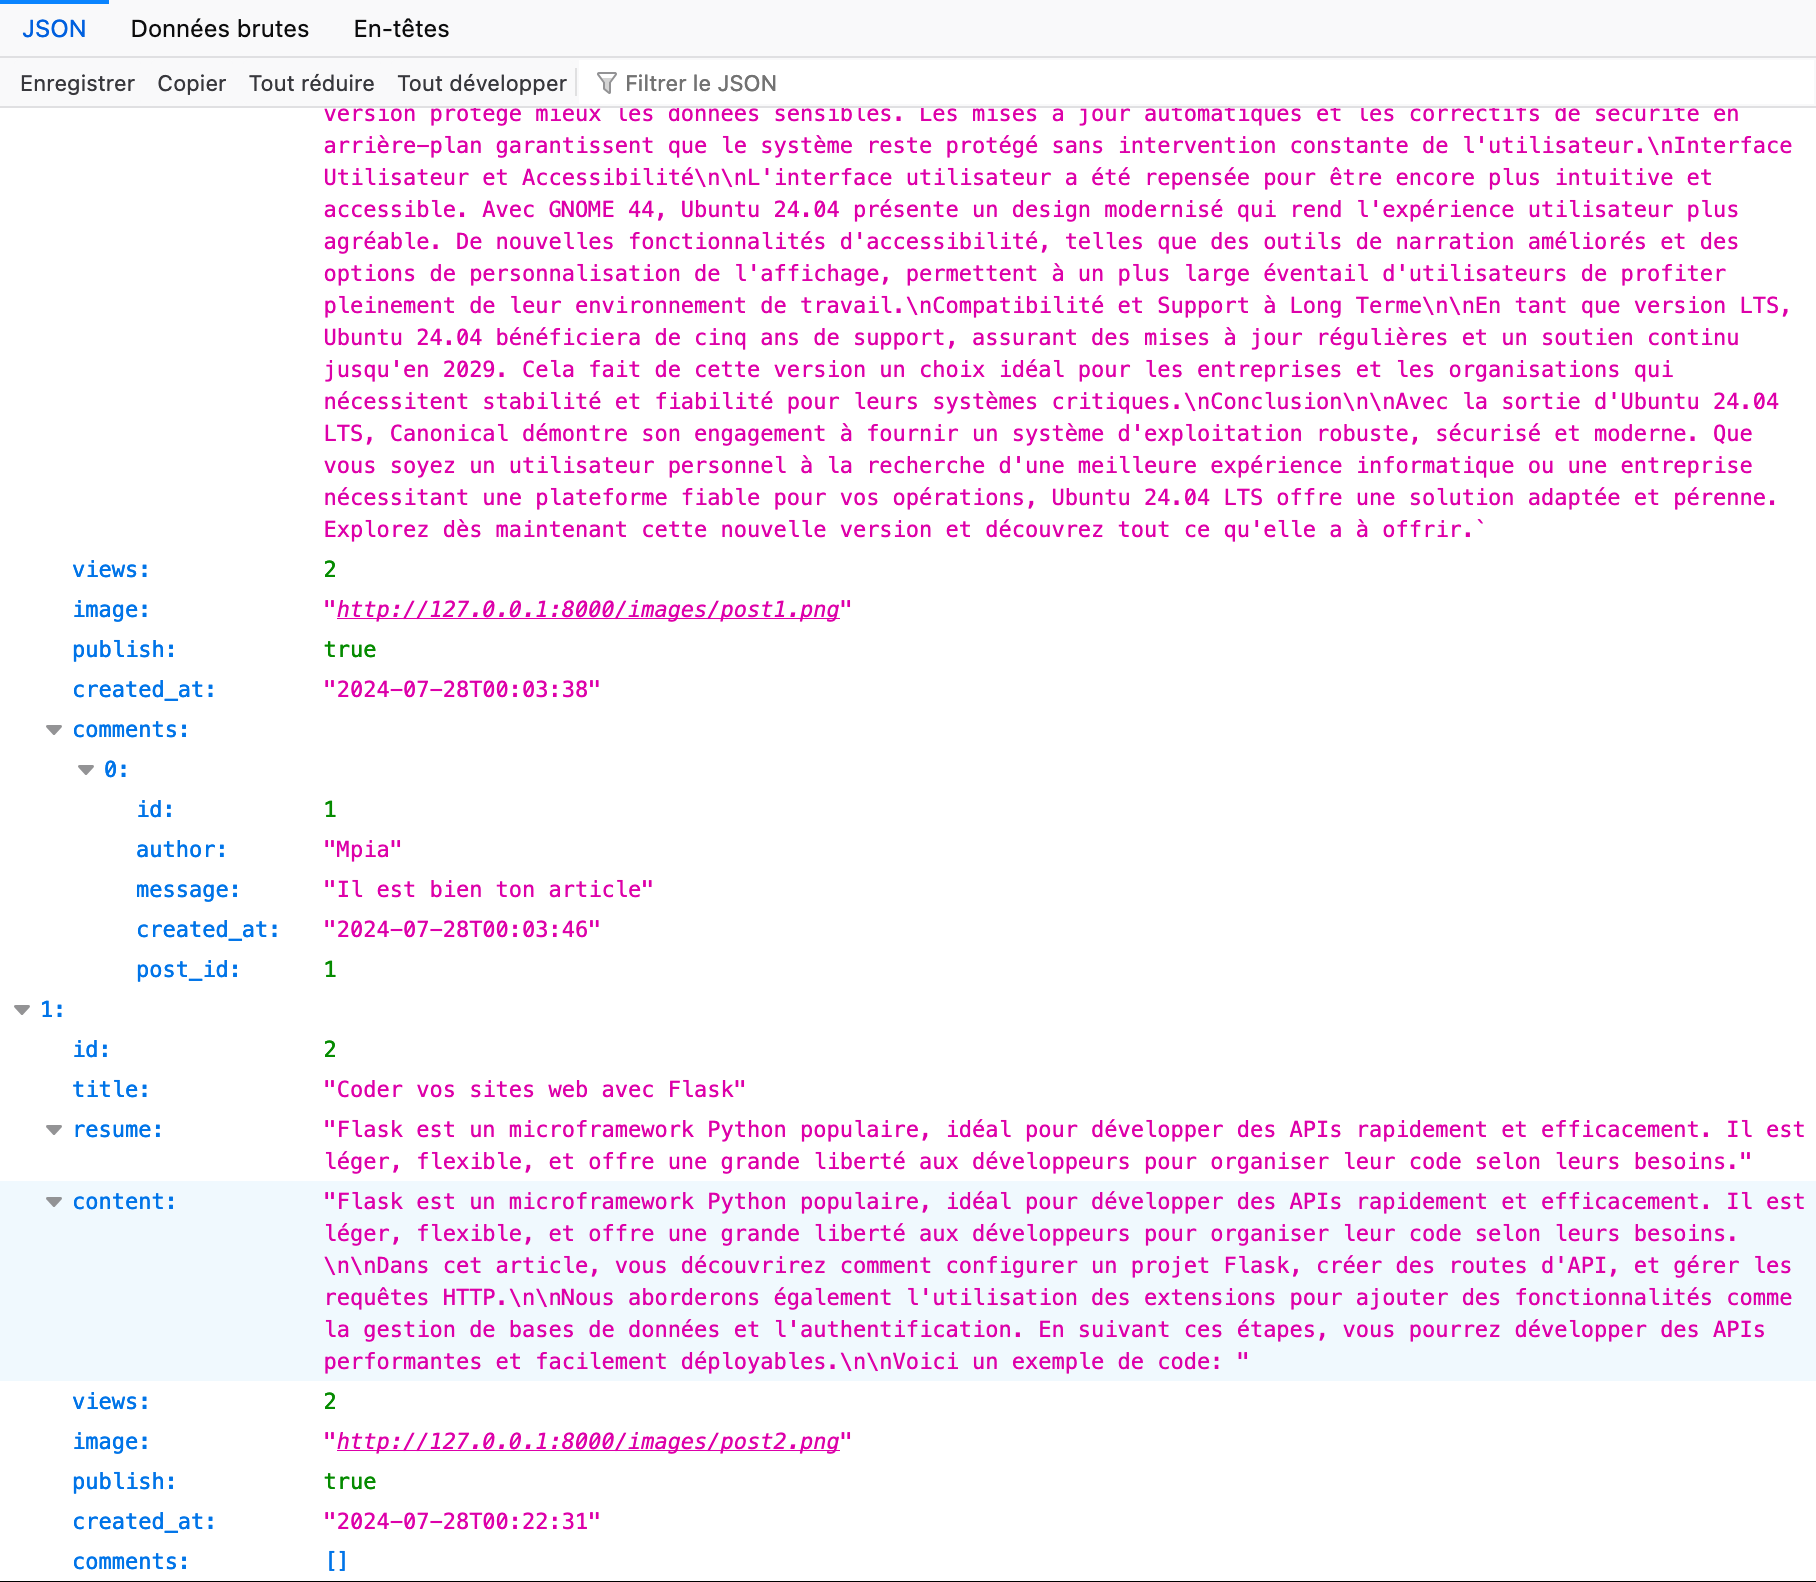
\includegraphics[width=0.8\textwidth]{TP-3/EXERCICE-3.1-A-RENDRE/screenshots/posts.png}
            \end{figure}
            
            \newpage
            \begin{figure}[ht]
                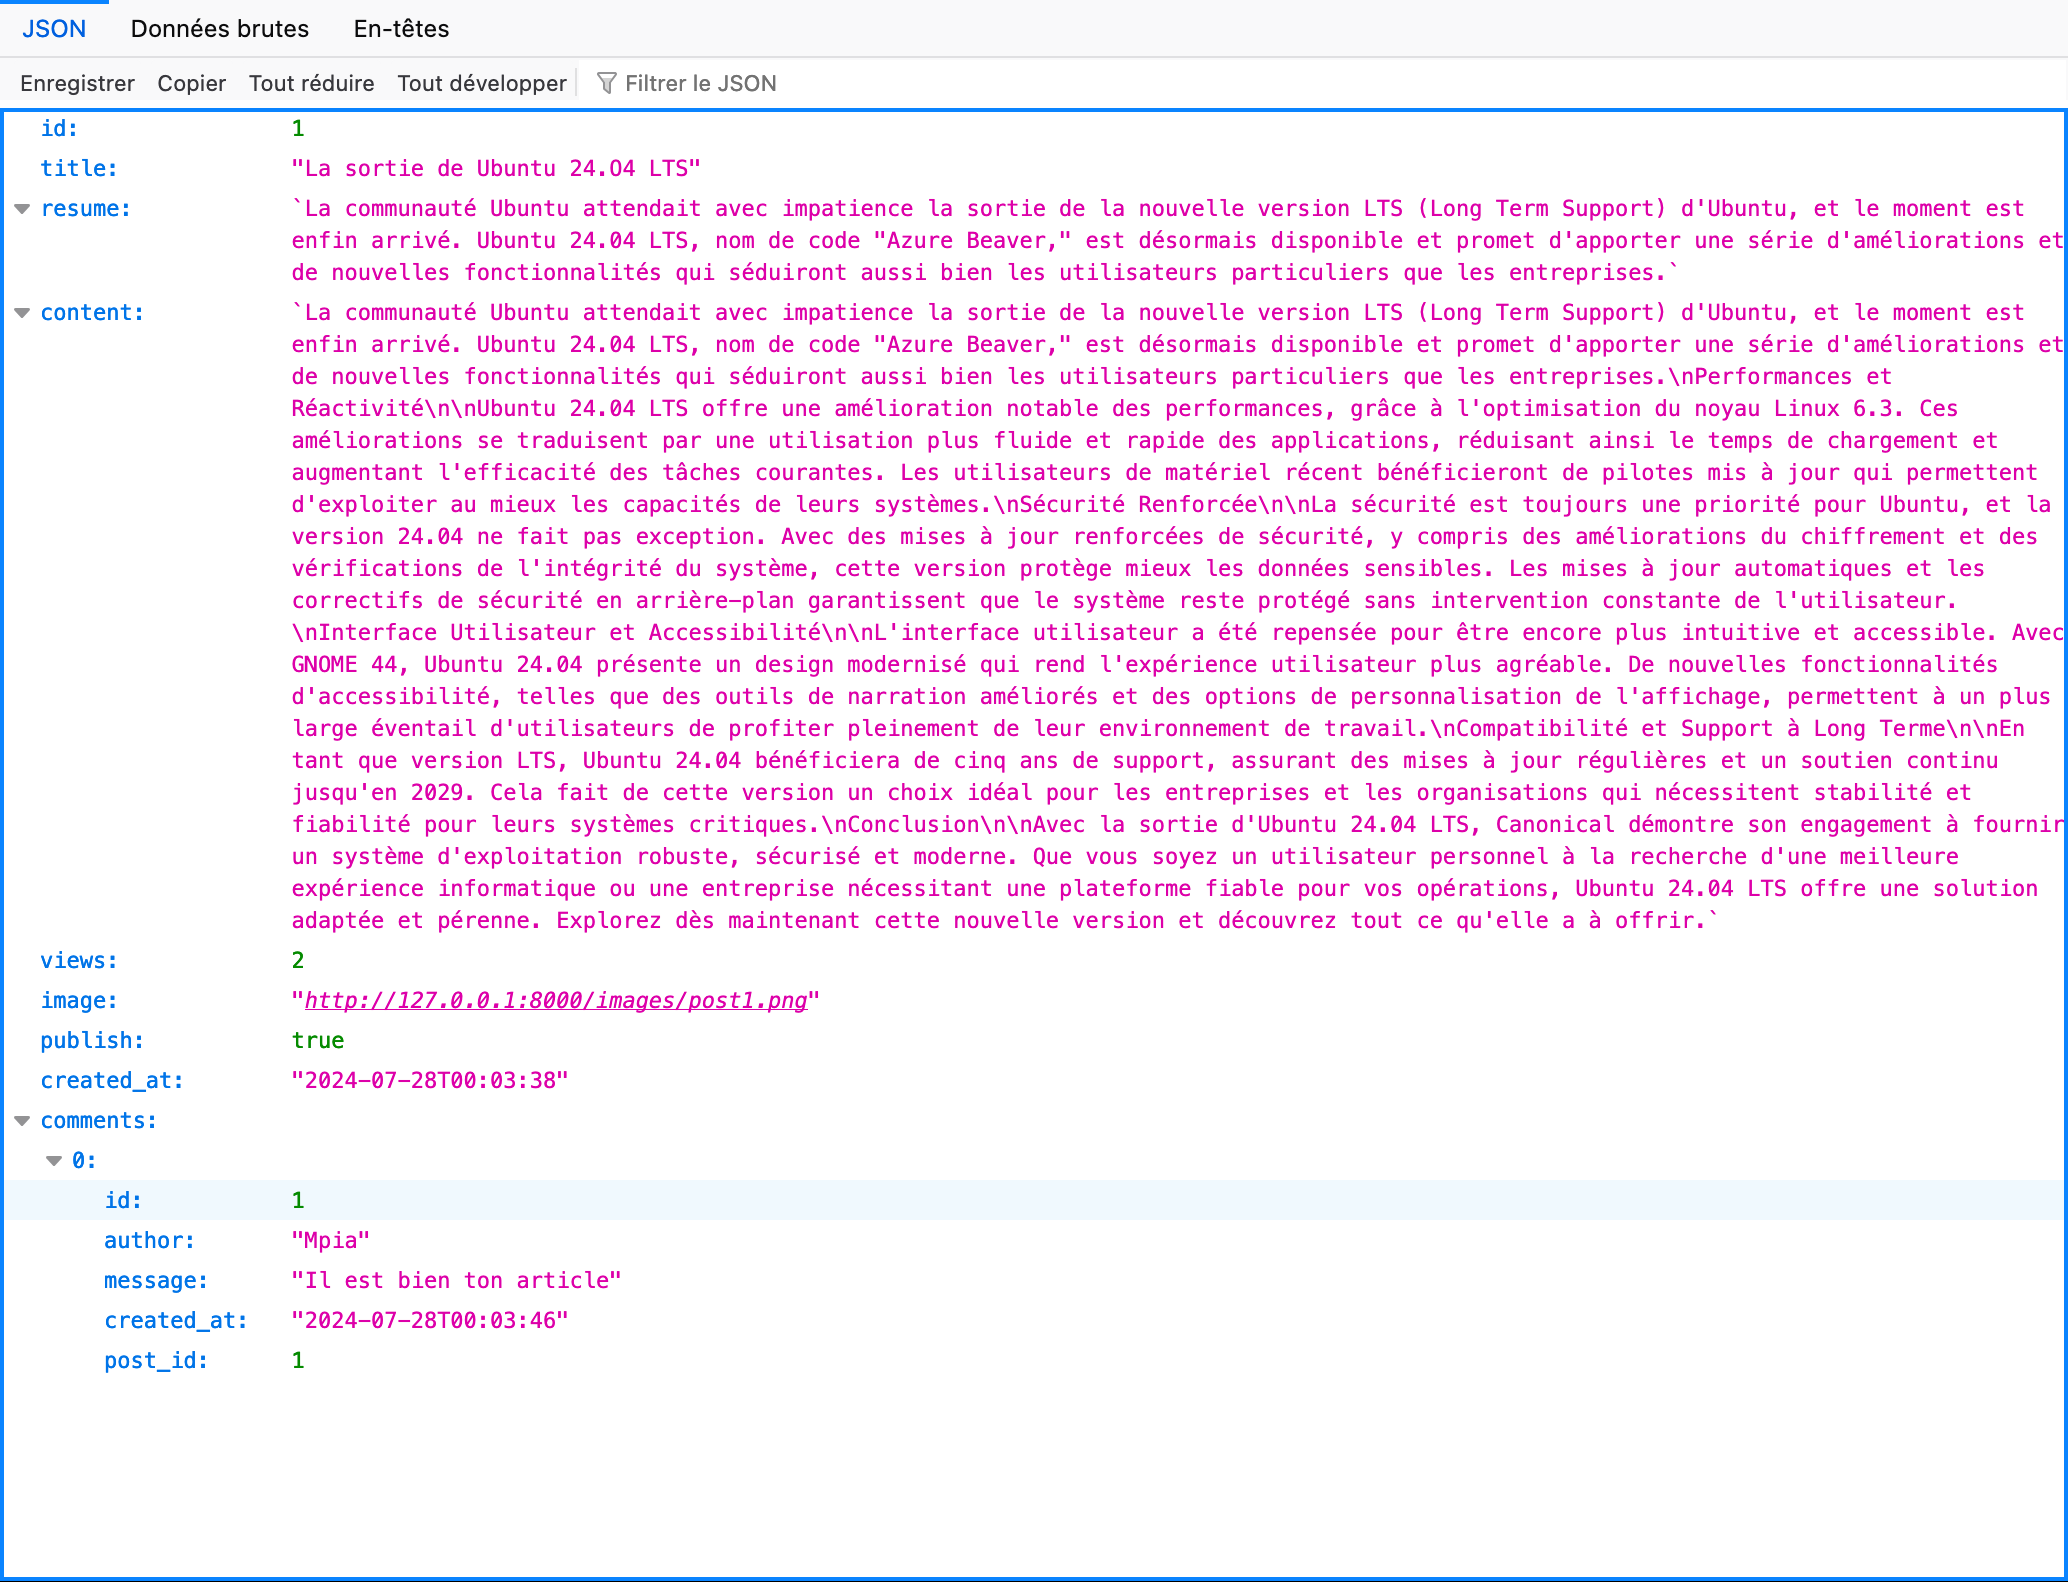
\includegraphics[width=0.8\textwidth]{TP-3/EXERCICE-3.1-A-RENDRE/screenshots/post.png}
            \end{figure}
            
        \begin{tcolorbox}[colback=lightgray!6, colframe=black, left=5mm, right=5mm, top=2mm, bottom=2mm, boxrule=0.1mm]
            La création d'une API avec FastAPI est un processus relativement simple et intuitif, grâce à la puissance et à la flexibilité de ce framework. 
            En utilisant FastAPI, nous avons pu définir des modèles de données avec Pydantic, interagir avec une base de données SQLite, et exposer des endpoints pour gérer les opérations CRUD (Create, Read, Update, Delete) sur les publications et les commentaires.\\

            FastAPI offre une documentation automatique via Swagger UI, ce qui facilite le test et la compréhension de l'API. De plus, il permet de gérer les requêtes asynchrones, ce qui peut améliorer les performances de l'application.\\

            En résumé, FastAPI est un excellent choix pour développer des API modernes et performantes. Sa simplicité d'utilisation, combinée à sa puissance et à ses fonctionnalités avancées, en fait un outil de choix pour les développeurs souhaitant créer des applications web robustes et évolutives.
        \end{tcolorbox}
    
    % TP 4
    \newpage
    \section{Quatrième partie:\\ TP 4 - Médias Immersifs, Réalité Virtuelle et Partages Collaboratifs}
        \subsection{Attendus de la partie 4}
            \noindent Pour ce quatrième et dernier TP, l’exercice 4.2 est à Rendre. L’exercice 4.3 qui vous demandera un peu de connaissances en Cryptographie et dans les "langages exotiques" est pour un Bonus orienté Mathématiques assez facile.
        
        \newpage
        \subsection{Exercice 4.2 (A Rendre)}
            \noindent \textit{En utilisant la plateforme Streamlit et votre espace (Repo) Github :
                \begin{enumerate}
                    \item Insérez une photographie (de vous, de Mnémosyne (cf GIL), de la personnalité de votre choix...) dans votre application Streamlit et générez un formulaire complet de manière à éditer (changer) un maximum de métadonnées EXIF (EXchangeable Image file Format) de cette image. Déposez votre code-source dans votre espace Github et lancez votre application en utilisant l’URL de celui-ci.
                    \item  Modifiez les données GPS (GPS tags) de votre photographie afin qu’elles correspondent à l’emplacement où vous vous trou- vez actuellement.
                    \item Pour vous aider, il existe un grand nombre de librairies Python à utiliser (Exif, ExifRead, la méthode getexif() de la Librairie PIL (Pillow),... ).
                    \item Affichez dans votre application Streamlit les coordonnées GPS saisies dans l’image sur une carte du pays correspondant à celles-ci.
                    \item Toujours dans une même application, dans une autre carte (ou plusieurs selon), affichez sous la forme de POI(s), tous les en- droits où vous vous êtes rendus (voyages, lieux d’habitation, ...) en les joignants entre eux. (Si vous n’avez pas ou peu voyagé, ajoutez les POI(s) des destinations de rêve que vous aimeriez visiter.)
                        - Pour vous aider, vous pouvez utiliser le composant Folium.
                        - N’oubliez pas d’illustrer vos réponses avec des C.E(s) illus- tratives, d’expliquer votre méthodologie et d’insérer et joindre vos codes python commentés.
                \end{enumerate}
            }
            \noindent Pour répondre à cet exercice, nous aurons besoin des modules Python suivants:
            \lstinputlisting{TP-4/EXERCICE-4.2-A-RENDRE/requirements.txt}

            \noindent Ils (modules) peuvent être installés en suivant les étapes suivantes:
            \begin{tcolorbox}[colback=lightgray!6, colframe=black, left=-40mm, right=5mm, top=2mm, bottom=-2mm, boxrule=0.1mm]
                \begin{verbatim}
                    # créer un env virtuel
                    python -m venv venv ou python3 -m venv venv 
                    # activer le vitualenv
                    source venv/bin/activate 
                    # Installer les modules
                    pip install -r requirements.txt ou pip3 install requirements.txt
                \end{verbatim}
            \end{tcolorbox}

            \noindent Maintenant que tout est prêt, voici le code de notre petite application Streamlit:

            \lstinputlisting{TP-4/EXERCICE-4.2-A-RENDRE/app.py}

            \noindent Cette application peut être lancée via la commande:
            \begin{tcolorbox}[colback=lightgray!6, colframe=black, left=-40mm, right=5mm, top=2mm, bottom=-2mm, boxrule=0.1mm]
                \begin{verbatim}
                    streamlit streamlit run
                \end{verbatim}
            \end{tcolorbox}

            \noindent Voici quelques captures d'écran:\\
            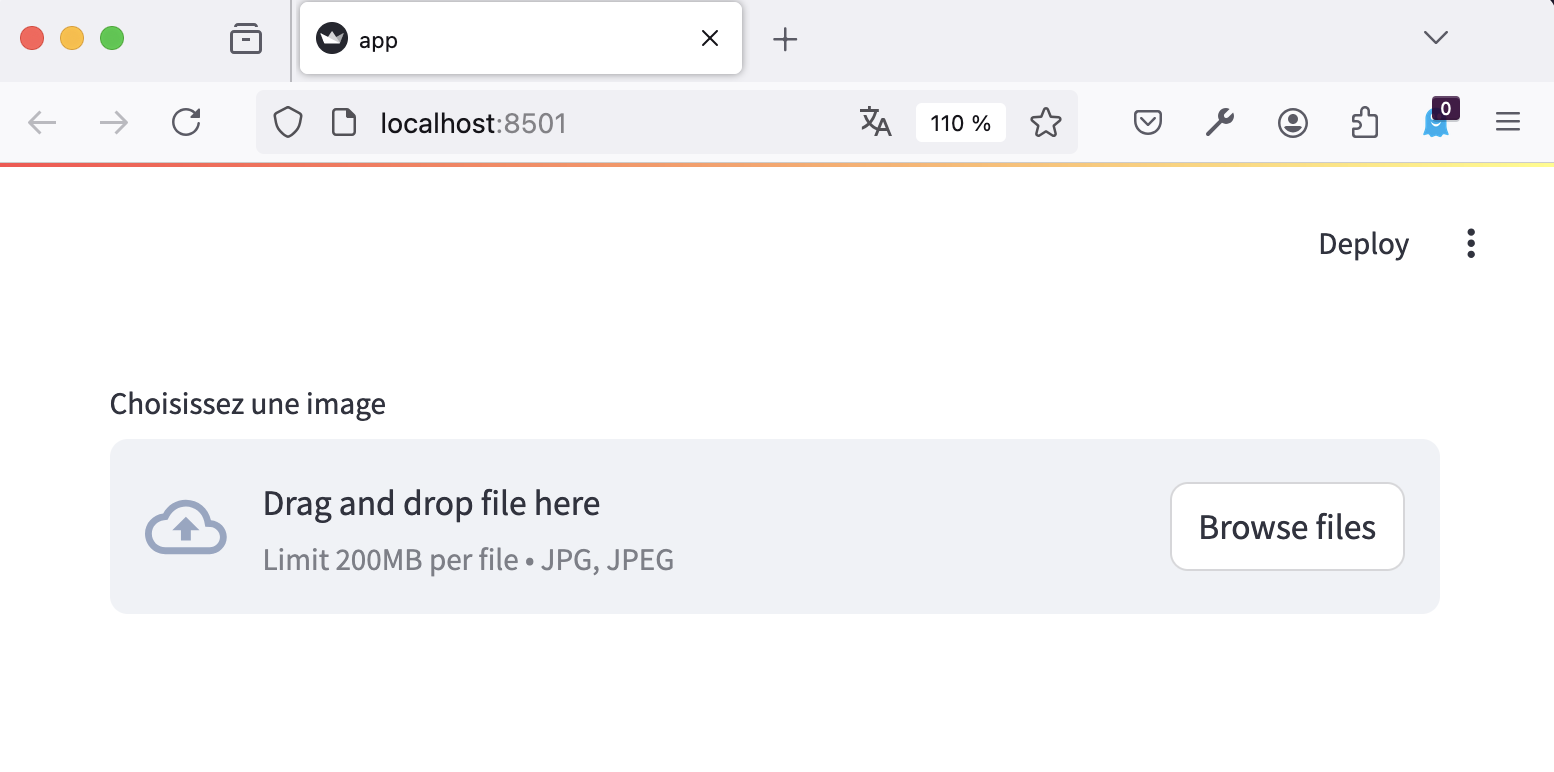
\includegraphics[width=0.8\textwidth]{TP-4/EXERCICE-4.2-A-RENDRE/screenshots/screen1.png}
            
            \newpage
            \includegraphics[width=0.5\textwidth]{TP-4/EXERCICE-4.2-A-RENDRE/screenshots/screen2.png}
            
        \newpage
        \subsection{Exercice 4.3 (Bonus)}
            \noindent Voici le décodage de toutes les consignes:
            \begin{enumerate}
                \item \textbf{Consigne 1}: \\
                    Créer une application Streamlit (la même que 4.2 ou une autre) qui cherche 
                    dans le premier million de décimales de PI la présence d'une date de naissance saisie par l'utilisateur.
                \item \textbf{Consigne 2}:\\
                    Dans un champ texte, après l'avoir calculé avec Python ou obtenu en ligne, affichez le jour de naissance correspondant.
                \item \textbf{Consigne 3}:
                    Dans un autre champ texte, calculer la somme des 20 premières décimales de PI, puis 
                    dans un second la somme des $12^2$ premières décimales ? Que remarquez-vous ?
                \item \textbf{Consigne 4}:
                    Insérez dans votre application une vidéo prise en ligne qui montre que la somme de tous les nombres naturels est égal à -1/12
            \end{enumerate}

            \noindent Pour réaliser une application Streamlit qui répond à ces 4 consignes, nous avons besoin de 2 modules:

            \lstinputlisting{TP-4/EXERCICE-4.3-BONUS/requirements.txt}

            \noindent Créons un environnement virtuel, activons-le et installons les modules.

            \begin{tcolorbox}[colback=lightgray!6, colframe=black, left=-40mm, right=5mm, top=2mm, bottom=-2mm, boxrule=0.1mm]
                \begin{verbatim}
                    # créer un env virtuel
                    python -m venv venv ou python3 -m venv venv 
                    # activer le vitualenv
                    source venv/bin/activate 
                    # Installer les modules
                    pip install -r requirements.txt ou pip3 install requirements.txt
                \end{verbatim}
            \end{tcolorbox}

            \noindent Voici le code complet de notre application:
            \lstinputlisting{TP-4/EXERCICE-4.3-BONUS/main.py}

            \noindent Une fois tous ces modules installés, nous pouvons lancer notre application, on faisant:
            \begin{tcolorbox}[colback=lightgray!6, colframe=black, left=-40mm, right=5mm, top=2mm, bottom=-2mm, boxrule=0.1mm]
                \begin{verbatim}
                    streamlit run main.py
                \end{verbatim}
            \end{tcolorbox}
        
        \newpage
        \noindent Voici la capture d'écran de cette application: 
        \begin{figure}[ht]
            \makebox[\textwidth][l]{
                \hspace{0.4cm}
                
\includegraphics[width=0.7\textwidth]{TP-4/EXERCICE-4.3-BONUS/screen1.png}
            }
        \end{figure}

        \begin{tcolorbox}[colback=lightgray!6, colframe=black, left=5mm, right=5mm, top=2mm, bottom=2mm, boxrule=0.1mm]
            En conclusion, nous avons créé une application Streamlit qui permet de rechercher une date de naissance dans les premières 1 million de décimales de PI, d’afficher le jour de la semaine correspondant, de calculer la somme des premières décimales de PI, et d’intégrer une vidéo expliquant un concept mathématique fascinant.
            Cette application démontre comment utiliser Python et Streamlit pour réaliser des tâches variées et interactives, tout en offrant une interface utilisateur simple et intuitive. Si vous avez d’autres questions ou souhaitez explorer davantage de fonctionnalités, n’hésitez pas à demander. Bonne exploration et programmation !
        \end{tcolorbox}
    
    % conclusion
    \newpage
    \section{Conclusion générale}
        \begin{tcolorbox}[colback=lightgray!6, colframe=black, left=5mm, right=5mm, top=2mm, bottom=2mm, boxrule=0.1mm]
            En résumé, les outils Git, GitHub et les API sont des éléments essentiels pour les développeurs et les équipes de développement moderne.\\ 
            
            - Git est un système de contrôle de version qui permet de gérer les changements dans le code, tandis que GitHub est une plateforme de collaboration en ligne qui permet de partager et de travailler sur des projets de code avec d'autres personnes.\\

            - Les API (Application Programming Interface) sont des interfaces de programmation qui permettent de communiquer avec des applications ou des services en ligne, ce qui permet de récupérer ou de transmettre des données de manière sécurisée et efficace.\\
            
            En combinant ces outils, les développeurs peuvent créer des workflows de développement efficaces, collaborer avec d'autres personnes sur des projets de code, et intégrer des services en ligne pour enrichir leurs applications.
        \end{tcolorbox}
\end{document}


